\documentclass[article]{aa}  
\usepackage{graphicx}
\usepackage{txfonts}
\usepackage[english]{babel}
\usepackage{amsmath}
\usepackage{amsfonts}
\usepackage{amssymb}
\usepackage{makeidx}
\usepackage{graphicx}
\usepackage{color}
\usepackage{appendix}
\usepackage{multirow}
%\usepackage[flushleft]{threeparttable}
%\usepackage{hyperref}
%\usepackage{nameref}

\newcommand{\derd}{{\rm d}}
\newcommand{\Log}{{\rm Log}}
\newcommand{\Ms}{{\rm M}_\odot}
\newcommand{\Zs}{{\rm Z}_\odot}
\newcommand{\au}{{\rm AU}}
\newcommand{\gw}{{\rm GW}}
\newcommand{\gc}{{\rm GC}}
\newcommand{\kl}{{\rm KL}}
\newcommand{\ibh}{{\rm IMBH}}
\newcommand{\imbh}{{\rm IMBH}}
\newcommand{\imri}{{\rm IMRI}}
\newcommand{\inn}{{\rm in}}
\newcommand{\out}{{\rm out}}
\newcommand{\bh}{{\rm BH}}
\newcommand{\bhu}{{\rm BH1}}
\newcommand{\bhd}{{\rm BH2}}
\newcommand{\ARGdf}{\texttt{ARGdf~}}
\newcommand{\ARCHAIN}{\texttt{ARCHAIN~}}

\newcommand{\manuel}{\textcolor{red}}
\newcommand{\pau}{\textcolor{blue}}
\newcommand{\xian}{\textcolor{green}}
\begin{document} 


\title{Formation and evolution of intermediate-mass ratio inspirals.}

\subtitle{Detecting intermediate-mass black holes in Milky Way globular clusters \\ and the Local Volume with LISA}

\titlerunning{Formation of IMRIs in Milky Way globular clusters and the Local Volume}	
\authorrunning{Arca Sedda, Amaro-Seoane, Chen}
\author{Manuel Arca Sedda \inst{1} \and Pau Amaro-Seoane \inst{2,}\inst{3,}\inst{4,}\inst{5} \and Xian Chen \inst{6,}\inst{5} }

\institute{Astronomisches Rechen-Institut. Zentrum f\"{u}r Astronomie der Universit\"{a}t Heidelberg, M\"onchhofstrasse 12-14, Heidelberg, D-69120, DE              
         \and         
			  Institute of Space Sciences (ICE, CSIC) \& Institut d'Estudis Espacials de Catalunya (IEEC) at Campus UAB, Carrer de Can Magrans s/n 08193 Barcelona, Spain
		\and         
			  Institute of Applied Mathematics, Academy of Mathematics and Systems Science, CAS, Beijing 100190, China
		\and
			  Zentrum f{\"u}r Astronomie und Astrophysik, TU Berlin, Hardenbergstra{\ss}e 36, 10623 Berlin, Germany
		\and         
			  Kavli Institute for Astronomy and Astrophysics at Peking University, Beijing 100871, P.R. China	
		\and
			Astronomy Department, School of Physics, Peking University, Beijing 100871, P.R. China	             
\\		\email{m.arcasedda@gmail.com}			
\\    	\email{pau@ice.cat}
\\		\email{xian.chen@pku.edu.cn }
}

\date{Received...; accepted...}


\abstract 
{The next generation of gravitational wave (GW) observatories would enable the detection of intermediate-mass black holes (IMBHs), an elusive type of black holes that are expected to lurk in the centre of massive clusters, dwarf galaxies and, possibly, AGN accretion discs. Intermediate mass ratio inspirals (IMRIs), composed of an IMBH and a compact stellar object, constitute one promising source of GWs audible to these detectors.} 
{We study the formation and evolution of IMRIs triggered by the interactions between two stellar BHs and an IMBH inhabiting the centre of a globular cluster, with the aim of placing constraints on IMRIs formation rate and detectability.}
{We exploit direct $N$-body models varying the IMBH mass, the stellar BH mass spectrum, and the star cluster properties. Our simulations take into account the host cluster gravitational field and General Relativistic effects via Post-Newtonian terms up to order 2.5.} 
{The chaotic dynamics involving the two BHs and the IMBHs has a significant impact on IMRIs formation: globally, the IMRIs formation probability attains values $\sim 5-50\%$, with larger values corresponding to larger IMBH masses. Merging IMRIs tend to map out the stellar BH mass spectrum, thus suggesting that their future detections can provide clues about the co-evolution of IMBHs and stellar BHs in star clusters. Given the post-merger GW recoil, we find that in typical globular clusters an IMBH with mass above $M_\ibh\sim 10^3\Ms$ have a retention probability above $50\%$ only if the companion mass is below $M_\bh\sim30\Ms$. Lower IMBHs, $M_\ibh \lesssim 200\Ms$, are expected to be ejected out of their cluster whenever the merging companion mass exceeds $M_\bh\sim 10\Ms$. Thus, localizing an IMBH in the center of a star cluster would give us insights on its past evolution. Our models show that the remnant spin encodes information about the IMBH evolution: at masses $M_\ibh = 10^2-10^3\Ms$ the final spin is strongly affected by the companion BH, whereas for $M_\ibh > 10^4\Ms$ the initial IMBH spin is preserved upon multiple mergers. Thus, depending on the IMBH mass, measuring the spin would shed a light on the IMBH evolutionary track. We show that IMRIs are powerful multiband sources that can be seen across different GW detectors during their last phases of life. We suggest that LISA can unravel the presence of IMBHs in Milky Way globular clusters, where the inferred signal-to-noise ratio (SNR) cumulated over 4 yr of observation is SNR$=10-100$, or in the Large Magellanic Cloud, for which we get an SNR$=8-40$. We infer the merger rate for several GW detectors, suggesting that LIGO should be able to see $0.9-2.5$ events per year involving an IMBH with mass $>100\Ms$, whereas LISA might detect $6-60$ events per year involving IMBHs as heavy as $4\times 10^4\Ms$. The next generation of detectors will shed further light on IMBHs: the Einstein Telescope can deliver up to $10^3$ events per year triggered by IMBHs with $M_\ibh \leq 2\times 10^3\Ms$, whereas DECIGO will allow $400-3800$ detections per yr involving $M_\ibh < 5\times 10^4\Ms$.}


\keywords{black hole physics --- gravitational waves ---  globular clusters: general --- Galaxy: general}

\maketitle
%
%-------------------------------------------------------------------

\section{Introduction}

Intermediate mass black holes (IMBH), with masses in the range $10^2-10^5\Ms$, might represent the missing link between stellar and supermassive mass black holes. Dense stellar systems, such as globular clusters (GCs), are thought to be ideal factories for IMBH production via formation and collapse of a very massive stars through stellar collisions \citep{zwart02, freitag06b,freitag06c, giersz15, mapelli16},
or via multiple interactions and mergers between stars and stellar-mass BHs \citep{giersz15}. Unfortunately, a striking observational evidence for the presence of IMBHs inhabiting GCs is still missing due to the little dynamical effects that these objects have on their surroundings \citep[for recent reviews see][]{mezcua17,greene19}. Indeed, models suggest that several processes can mimic an IMBH, like anisotropies inthe GC kinematic  properties \citep{zocchi}, or the presence of a dense cluster of stellar mass BHs -- namely a BH subsystem -- that dominate the inner cluster centre \citep{AAG18b,AS16,vandermarel10}. Nevertheless, a few observational IMBHs candidates have been found for Galactic GCs
\citep{noyola10,lu13,lanzoni13,kiziltan17} and their mass and influence radius might be possibly connected with the host cluster observational 
properties \citep{AAG18a}. Due to this, finding an unique way to unravel the presence of IMBHs in GCs represents one of the most interesting challenges in modern astronomy. Beside this, the presence of an IMBH sitting in the centre of a dense cluster represents a scenario particularly appealing from the perspectives of gravitational waves (GW) astronomy. Indeed, a compact remnants orbiting the IMBH can enter a regime where GWs emission dominates, leading to the formation of an intermediate mass-ratio inspiral \citep[IMRI,][]{konstantinidis13,leigh14,haster16,macleod16}, a class of sources possible audible with the next generation of GW observatories like LISA \citep{seoane07,amaro12,seoane18}. However, in the highly dense regions that characterize star clusters centres, the formation of IMRIs is not a smooth process. Indeed, due to the continuous interactions with stars, an IMRI ``progenitor'', namely a tight IMBH-BH binary, might be subjected to strong perturbation induced, for instance by a passing-by BH. The three-body interaction involving the IMBH and the two BHs can lead to a variety of end states, including the formation of an IMRI, a stellar BH binary, the ejection of one BH, or even both, or the development of a head-on collision. At some extent, this scenario is similar to what is expected to happen in galactic nuclei, where supermassive BHs (SMBHs) can capture a compact object to form an extreme mass ratio inspiral. However, in the case of IMRIs the picture is complicated by the fact that this chaotic process can transfer to the IMBH an amount of energy sufficient to displace it sensibly from the cluster centre. Differently from galactic nuclei, where the SMBH remains well seated in the galactic potential well, the IMBH motion makes hard the use of any analytical approach to solve IMRIs dynamics. Quantifying the branching ratio for IMRIs formation constitute a fundamental step to assess the probability to observe these GW sources with the next generation of space-based detectors like LISA\footnote{\url{https://www.elisascience.org/}} \citep{seoane07,amaro12}, TianQin \citep{tianqin16} or Taiji \citep{taiji17}. In this paper, we model the potential formation of an IMRI from the interactions between an IMBH and two stellar mass BHs. This type of  configuration can temporarily form in the centre of clusters with IMBH mass $\sim 100-1000\Ms$ \citep{konstantinidis13,macleod16} and could last up to $10^7$ yr \citep{macleod16} although this depends strongly on the cluster initial properties. In fact, it is difficult to predict the actual amount of BHs that, at any time, interact with the IMBH, primarily because the majority of the studies conducted in the literature assume that the IMBH is already at the centre of the host cluster when stellar BHs form and sink toward the cluster centre \citep{leigh14,haster16}. Models in which the IMBH is a byproduct of stellar evolution and collisions, indeed, seem to point out that after the IMBH grows only a handful of stellar BHs are still present in the cluster $<3-5$ \citep{AAG19}. To reach the aim, we use $N$-body simulations that take into account in particles' equations of motion both the star cluster gravitational potential and post-Newtonian corrections at 1, 2, and 2.5 order. Varying the IMBH and BHs masses, their orbital configuration, and the host cluster structural properties, we build-up three sets consisting of 2000 models each, which allow us to uncover three possible scenarios for IMRIs formation.  
The paper is organized as follows: in Section \ref{num} we
present and summarize the numerical setup used to model the IMBH - BH
interaction, in Section \ref{res} we present and discuss the main properties of
the simulations output, in Section \ref{gra} we discuss the implications for GW
astronomy, while Section \ref{res} is devoted to the results summary and
conclusions. 





\section{Initial conditions} 
\label{num}


{\bf
We simulate the evolution of the innermost region of the cluster, modelling the IMBH and two stellar mass BHs as live particles and
the remaining cluster as an external static potential. In order to explore the parameter space, we create six different models, each one consisting 
of 4000 simulations gathered in four different sub-classes, depending on the IMBH mass, for a total of 48,000 simulations. Our model is sketched in Figure \ref{f1}. 

\begin{figure}
    \centering
    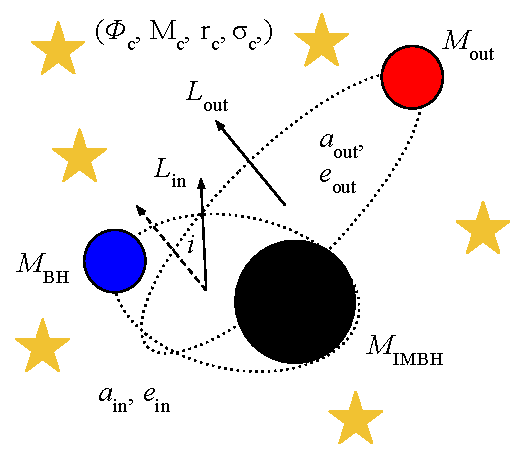
\includegraphics[width=7cm]{triple}
    \caption{Sketch of the IMBH-BH-BH triple configuration.}    
\label{f1}
\end{figure}

We vary the central IMBH mass in four classes, namely ${\rm Log}(M_\ibh/\Ms) = 2-3-4-5$. This range covers typical values of putative IMBH masses forming in stellar systems of various sizes, from young and open clusters, to globular clusters, and up to low-mass nuclear clusters and dwarf galaxies.
We note that the lowest value taken for $M_\ibh$ will likely involve mergers with mass ratio $> 0.1$, thus they fall outside the range of IMRIs. Nonetheless, exploring the low end of IMBH mass function will help us in better understanding the perspectives of IMBH-BH mergers from the point of view of both low- and high-frequency GW detectors, as discussed in Section XX.

The properties of the cluster in which the IMBH is embedded, which define the cluster potential, are varied depending on the model. The cluster density profile is assumed to be either a Dehnen sphere with inner slope $\gamma_\gc = 0.5$ (model S0, S3, S4, S5, S6) or $1.0$ (model S1), or a Plummer sphere (model S2). In both cases, the cluster half-light radius is assumed to be $R_{\rm eff} = 3.4$ pc, namely the mean value of Milky Way globular clusters \citep{harris14}. The mass of the cluster is calculated via the scaling provided by \cite{AS16}, connecting the host cluster mass $M_\gc$ with the total ``dark'' mass, inhabiting the cluster's centre, comprised of either an IMBH or a sizable population of stellar BHs
\begin{equation}
\Log \left(\frac{M_\gc}{\Ms}\right) = \alpha \Log \left(\frac{M_\ibh}{\Ms}\right) + \beta.
\label{mcmibh}
\end{equation}
with $\alpha = 0.999 \pm 0.001$ and $\beta = 2.23 \pm 0.009$. The cluster typical radius is thus calculated from the assumed $R_{\rm eff}$ and the adopted mass profile. Upon these assumptions an IMBH with mass $M_\ibh = 10^2(10^5)\Ms$ is associated with a cluster mass of $ M_\gc = 1.7\times 10^4(1.7\times 10^7)\Ms$, thus our models ideally span the mass range of young clusters, globular clusters, and dwarf galaxies nuclei. We assume that the IMBH is orbited by two stellar BHs, since the IMBH is expected to be the most massive object in the cluster and the dominant element in determining the dynamics. The orbital eccentricity $e_{1,2}$ is extracted randomly according to a thermal distribution $P(e){\rm d} e = 2e{\rm d}e$, while the semimajor axis $a_{1,2}$ is selected according to the overall cluster density profile with the exception of model S6, in which we extract $a_{1,2} = 0.1-10^4$ AU assuming a distribution flat in logarithmic values.  
In models S0 to S5, the maximum semimajor axis allowed is set equal to the radius within which the host cluster contains two stellar BHs with average mass $30\Ms$. 

The BH mass spectrum is also allowed to vary: we use the BH mass spectrum derived by \citep[SM17][]{spera17}, assuming a progenitor metallicity of $Z = 0.0002$ for models S0, S1, S2, and S5 and $Z = 0.02$ for model S6; a power-law mass spectrum with slope $2.2$ \citep[O16][]{oleary16} in the range $3-30 \Ms$ (model S3); or a flat distribution in the range $3-30 \Ms$ (hereafter FLAT, model S4). The three different BH mass spectrum adopted describes two possible situations, one in which the BH population reflect the original population of stars and another in which dynamics operated a selection on the BH mass distribution either mild (power-law distribution) or sufficiently strong to erase any memory of the original mass function (flat distribution). 
}


\begin{table*}
\caption{Main properties of our models}
\begin{center}
\begin{tabular}{cccccccccccc}
\hline
\hline
ID & $M_\ibh$ & $M_\gc$ & $\rho_\gc$ & $\gamma_\gc$ & $a$ &$e$ &BH & $m_{\bh, min/max}$ & $Z$ & $N_{\rm sim}$ \\ 
   & $\Ms$    & $\Ms$   &            &              &     &    &   & $\Ms$              &     & \\
\hline
S0 & $10^2-10^5$ & $1.7\times 10^4 - 1.7\times 10^7$ & Dehnen & $0.5$ & density & thermal & SM17 & $4-53.4$ & 0.0002 & 1,000 $\times$ 4 \\
S1 & $10^2-10^5$ & $1.7\times 10^4 - 1.7\times 10^7$ & Dehnen & $1.0$ & density & thermal & SM17 & $4-53.4$ & 0.0002 & 1,000 $\times$ 4 \\
S2 & $10^2-10^5$ & $1.7\times 10^4 - 1.7\times 10^7$ & Plummer& $0.0$ & density & thermal & SM17 & $4-53.4$ & 0.0002 & 1,000 $\times$ 4 \\
S3 & $10^2-10^5$ & $1.7\times 10^4 - 1.7\times 10^7$ & Dehnen & $0.5$ & density & thermal & O+16 & $3-30$ & 0.0002 & 1,000 $\times$ 4 \\
S4 & $10^2-10^5$ & $1.7\times 10^4 - 1.7\times 10^7$ & Dehnen & $0.5$ & density & thermal & FLAT & $3-30$ & 0.0002 & 1,000 $\times$ 4 \\
S5 & $10^2-10^5$ & $1.7\times 10^4 - 1.7\times 10^7$ & Dehnen & $0.5$ & logflat & thermal & SM17 & $4-53.4$ & 0.0002 & 1,000 $\times$ 4 \\
S6 & $10^2-10^5$ & $1.7\times 10^4 - 1.7\times 10^7$ & Dehnen & $0.5$ & density & thermal & SM17 & $4-53.4$ & 0.02   & 1,000 $\times$ 4 \\
\hline
\end{tabular}
\label{tabt1}
\end{center}
\end{table*}

{\bf 
All simulations are performed taking advantage of \ARGdf \citep{ASCD19}, a modified version of the \ARCHAIN code that implements post-Newtonian (PN) dynamics and {\it algorithmic regularization} to handle close encounters and strong collisions \citep{mikkola99,mikkola08}. For our purposes, we include in our treatment only 1, 2, and 2.5 order PN terms. Additionally, \ARGdf allows the user to take into account in particles' equations of motion the gravitational field generated by the host stellary system and a dynamical friction term. Simulations are halted either if one of the two BH merge with the IMBH, if one of the BHs is ejected away if the simulated time exceeds $t = 1$ Gyr, or if the runtime exceeded 1 hr. The $1$ Gyr time limit serves to cope with the fact that IMBH in the range of masses $>10^3\Ms$ are expected to build-up via stellar accretion and mergers with compact remnants over timescales that can range considerably $1-10$ Gyr depending on the formation pathway \citep[see for instance][]{giersz15}. A summary of all models considered is provided in Table \ref{tabt1}.
}

\section{Results}
\label{res}

\subsection{IMRIs formation and merger}
\label{sec:imris}


\begin{figure*}
    \centering
    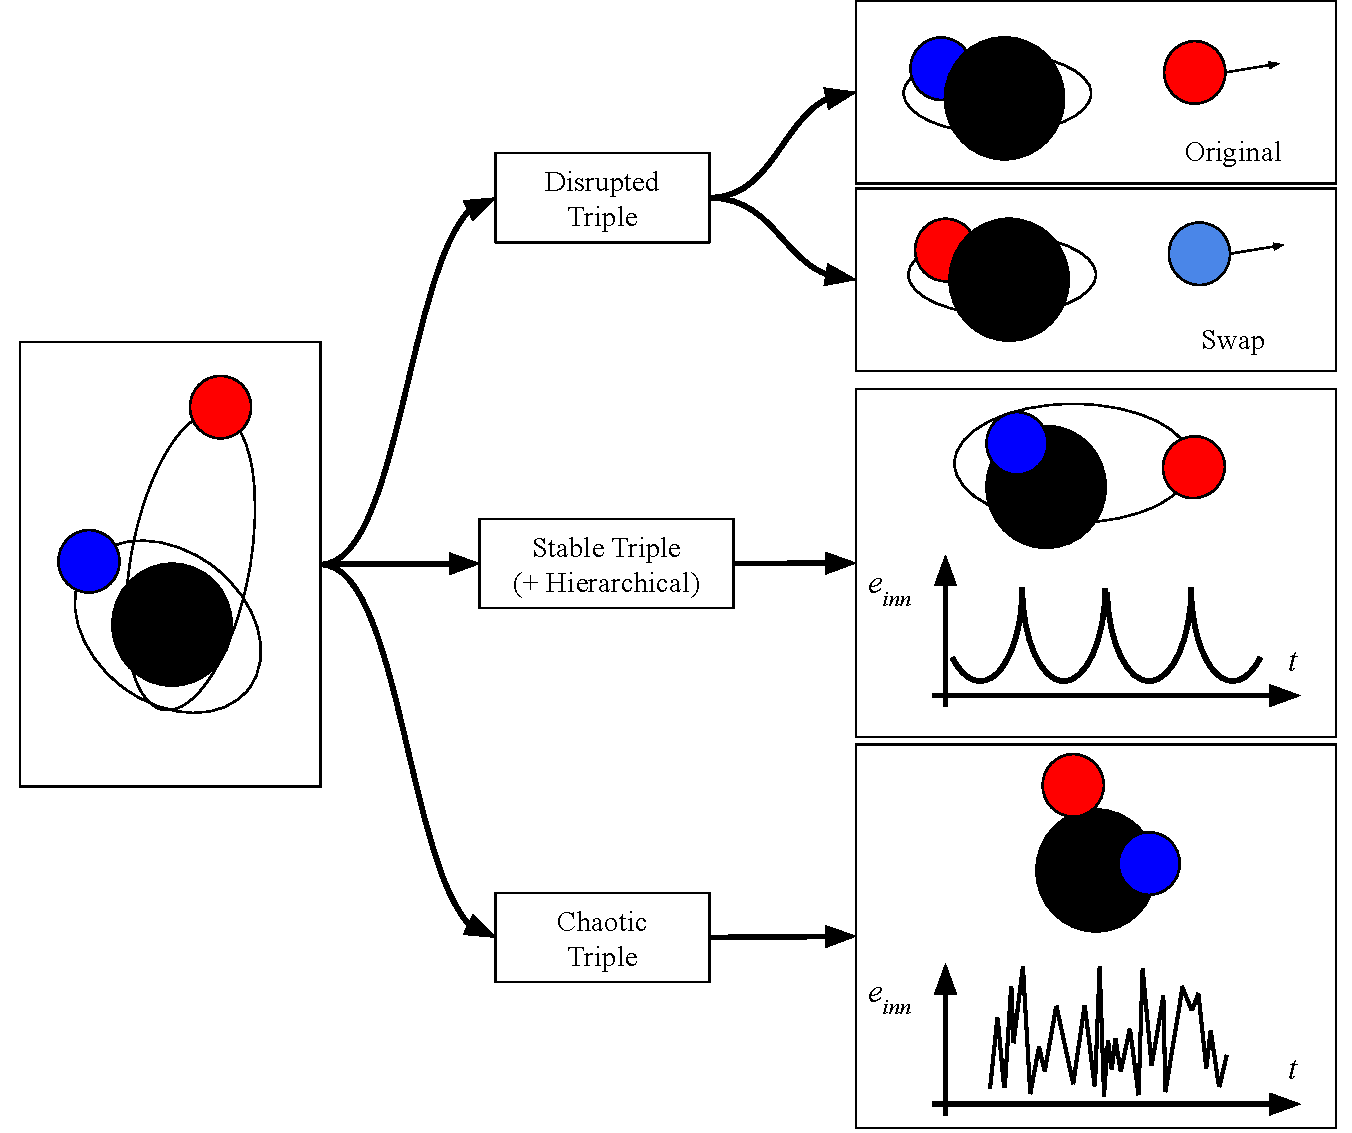
\includegraphics[width=16cm]{Sketch_IMRI}
    \caption{Schematic view of IMBH-BH-BH triple evolution.}
    \label{fig:f3}
\end{figure*}

\begin{table*}
\caption{Main results of $N$-body simulations}
\label{tab:mergers}
%\centering{}
\begin{center}
\begin{tabular}{c|cccc|cccc}
\hline
\hline
ID   & $f_{\rm bnd}$ & $f_{\rm dis}$ & $f_{\rm mer}$ & $f_{\rm mer,d}$ & \multicolumn{4}{c}{$f_{\rm mer,ibh}$} \\
     & $\%$          & $\%$          & $\%$         & $\%$          & \multicolumn{4}{c}{$\%$}\\
     &               &               &              &               &$10^2\Ms$&$10^3\Ms$&$10^4\Ms$&$10^5\Ms$\\
\hline
S$0$ & $25.73$ & $47.77$ & $26.50$ & $2.08$ & $3.1 $ & $28.6 $ & $51.6 $ & $30.9 $ \\ 
S$1$ & $21.88$ & $58.12$ & $20.00$ & $2.33$ & $3.5 $ & $28.5 $ & $38.7 $ & $18.6 $ \\ 
S$2$ & $39.17$ & $36.08$ & $24.75$ & $0.28$ & $0.0 $ & $11.7 $ & $43.6 $ & $44.8 $ \\ 
S$3$ & $28.68$ & $40.05$ & $31.27$ & $1.15$ & $5.5 $ & $48.6 $ & $43.6 $ & $31.7 $ \\ 
S$4$ & $26.70$ & $44.88$ & $28.43$ & $2.08$ & $3.4 $ & $38.8 $ & $49.0 $ & $30.8 $ \\ 
S$5$ & $40.48$ & $41.03$ & $17.70$ & $29.35$& $30.5 $ & $42.5 $ & $50.1 $ & $64.8 $ \\ 
S$6$ & $29.57$ & $37.80$ & $32.62$ & $1.43$ & $3.6 $ & $50.3 $ & $49.2 $ & $33.1 $ \\ 
\hline
\end{tabular}
\label{tab:t2}
\end{center}
\end{table*}

{\bf

In this section we discuss the main results of our simulations. In the following, we refer indifferently to IMBH-BH and IMRI although the smallest value of the IMBH mass adopted ($10^2\Ms$) leads to IMBH-BH mergers with a mass ratio larger than expected for IMRIs. We discuss the implication for GW astronomy in the next section. 

The outcomes of our simulations can be classified in three main categories: 
\begin{itemize}
\item[a)] the IMBH-BH-BH system remains bound over the simulated time ({\it bound});
\item[b)] one of the stellar BHs is ejected away leaving behind an IMBH-BH binary ({\it disrupted}); 
\item[c)] one of the BH merges with the IMBH ({\it mergers}). 
\end{itemize}
Figure \ref{fig:f3} provides a simplistic sketch of the possible outcomes of our simulations. Table \ref{tab:t2} shows the percentage of models falling in each of these categories for the different models explored. On average, we note that mergers constitute the $f_{\rm GW} \sim 20-32\%$ of models, with little dependence on the initial conditions assumed. 
Models falling in category a) or b) do not exclude automatically an IMBH-BH merger. In case a), i.e. a bound IMBH-BH-BH, the triplet can arrange in a configuration in which the IMBH forms a tighter bound with one of the BHs while the other orbits around their common centre of mass. In this case, the triple can either evolve chaotically or undergo secular effects like the so called Kozai-Lidov mechanism \citep{kozai62,lidov62} that can trigger the eccentricity of the innermost IMBH-BH binary to grow to values close to unity. 

In case b), i.e. ejection of one of the stellar BHs, the evolution of the remaining IMBH-BH binary will be due to the sum of two contributes, namely energy removal from binary-single interactions and GW emission. The first contribute compromise the IMBH-BH survival over a typical {\it evaporation time} \citep{bt,stephan16,hoang18} 
\begin{align}
t_{\rm ev} =& \frac{\sqrt{3}\sigma_g}{32\sqrt{\pi}G\rho_g\ln\Lambda a} \frac{m}{m_*} = \nonumber \\
            & 1.3\times 10^{10} {\rm ~yr} 
            \left(\frac{\sigma_g}{5{\rm ~km~s^{-1}}}\right)
            \left(\frac{10^5{\rm ~M}_\odot ~pc^{-3}}{\rho_g}\right) \times \nonumber \\
            & \times \left(\frac{0.1{\rm ~AU}}{a}\right)\left(\frac{1030{\rm ~M}_\odot}{M_{\rm ibh}+M_{\rm bh}}\right)\left(\frac{m_*}{30{\rm ~M}_\odot}\right),
\label{eva}
\end{align}
where $m_*$ is the average stellar mass in the nucleus, $\rho_g$ is the stellar density, $\sigma_g$ is the cluster velocity dispersion, and $\ln\Lambda=6.5$ is the Couloumb logarithm. If the IMBH-BH entered the IMRI phase, binary-single interactions are expected to play little to no effect on its evolution \citep{seoane18}. In this case, the IMRI will continuously shrink emitting GWs until coalescence, which takes place on a timescale \citep{peters64}
\begin{align}
t_\gw =&  \displaystyle \frac{5}{256}\frac{c^5 a_\inn^4 (1-e_\inn^2)^{7/2}}{G^3M_\ibh M_\bh(M_\ibh+M_\bh)} = \nonumber \\
       & 10^6{\rm ~yr}\left(\frac{a_\inn}{0.1\au}\right)^4\left(1-e_\inn^2\right)^{7/2}\times \nonumber \\ 
       & \times \left(\frac{10^3\Ms}{M_\ibh}\right) \left(\frac{30\Ms}{M_\bh}\right)\left(\frac{1030\Ms}{M_\ibh+M_\bh}\right).
\label{peters}
\end{align}
In principle, a binary having $t_\gw < t_{\rm ev}$ is most likely to merge before dynamical encounters manage to break it.
Therefore, as summarized in Table \ref{tab:t2}, among all models we calculate both the percentage of ``direct mergers'' $f_{\rm mer}$ -- mergers that happen before the simulations end -- and ``delayed mergers'' $f_{\rm mer,d}$ -- i.e. IMBH-BH binaries that satisfy the $t_\gw < t_{\rm ev}$ criterion. The amount of delayed mergers represents about $0.2-2.3\%$ of the simulated cases. 

Clearly, while the categorization provided suggests three well separate classes, it must be noted that models falling in case c) (mergers) might have undergone a chaotic triple phase, or secular effects that triggered the IMBH-BH merger. In fact, figure \ref{fig:example} shows a typical example of one of the simulations performed in which the merger takes place within the simulated time. In the example, an IMBH with mass $M_\ibh = 10^2\Ms$ forms a tight binary with a stellar BH with mass $M_\bh = 15\Ms$, the binary is subjected to perturbation of the outer BH with mass $M_\bh = 5\Ms$ that causes a continuous oscillation of the eccentricity up to the point -- around 300 Myr from the beginning of the simulation -- at which the eccentricity peaks at values $\sim 0.999998$ and GW start dominating the IMBH-BH binary evolution which culminate with a merger shortly after.  
}
\begin{figure}
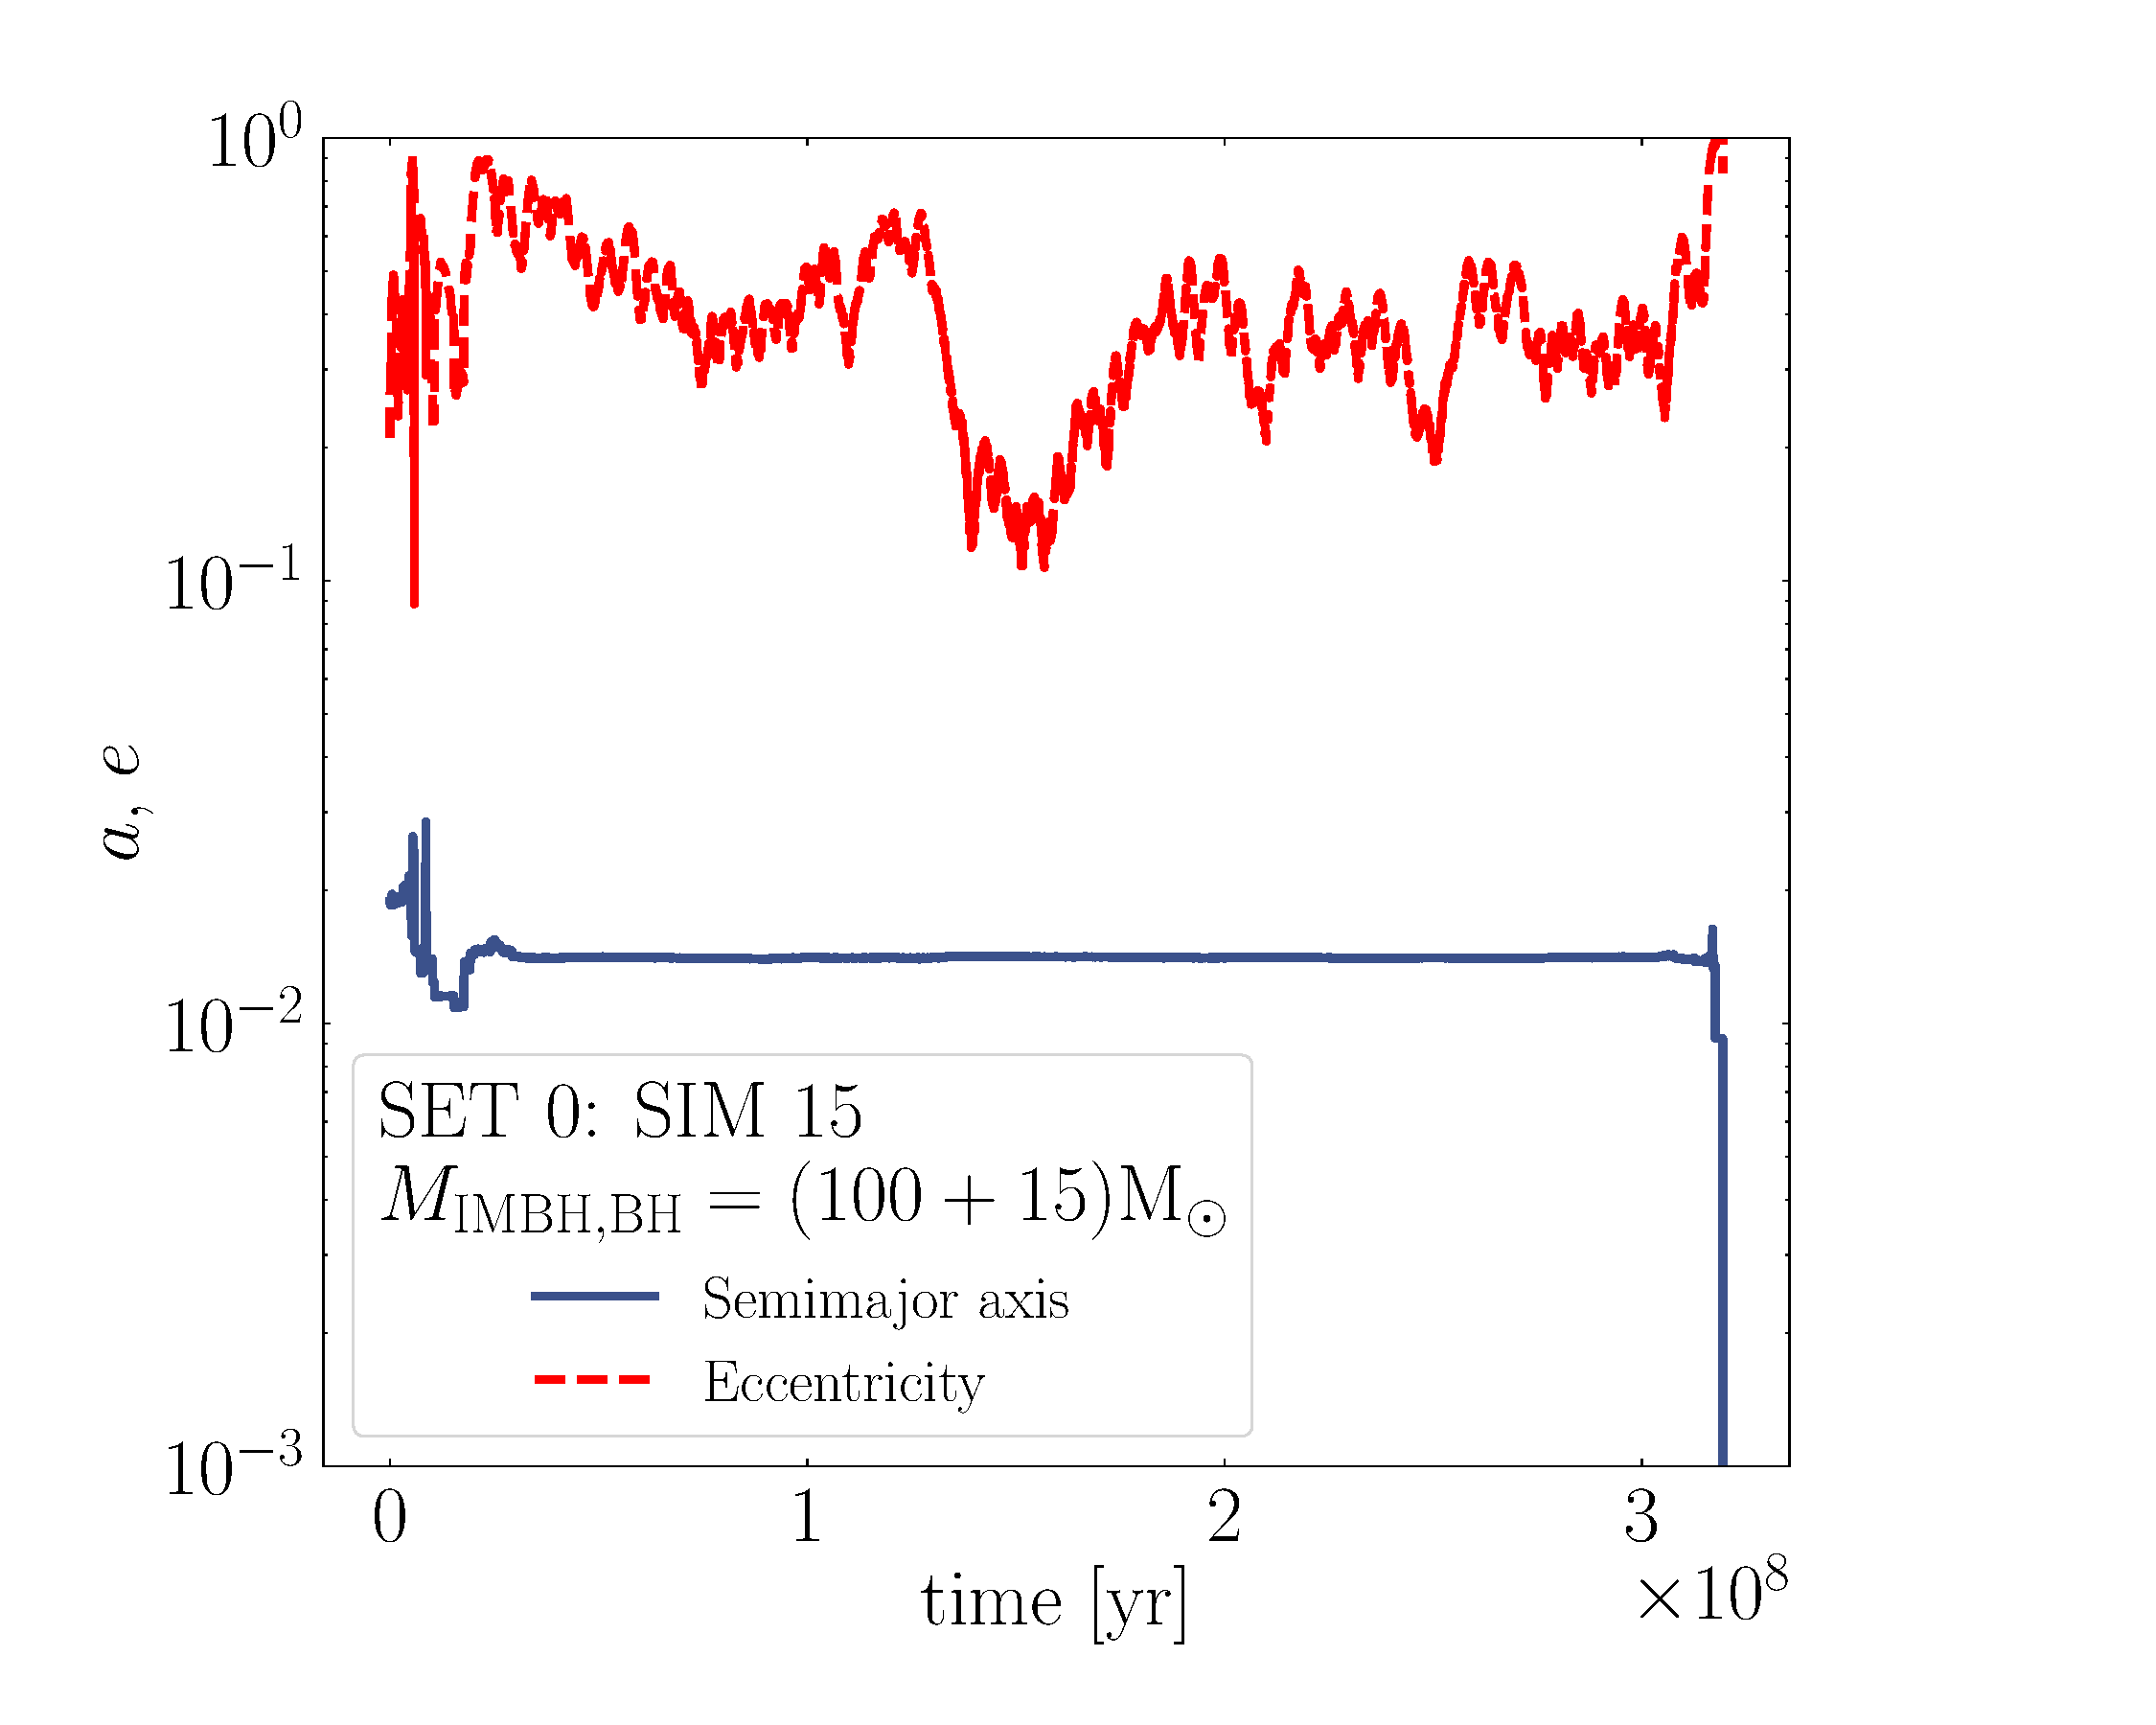
\includegraphics[width=\columnwidth]{example}
    \caption{Time evolution of the semimajor axis (straight blue line) and eccentricity (dotted red line) for one of the simulations performed in SET0.}
	\label{fig:example}
\end{figure}


{\bf 

The amount of both ``direct'' and ``delayed'' merger depends, as outlined in Table \ref{tab:t2}, on the IMBH mass and the model investigated. Figure \ref{fig:gwprob} shows the percentage of total mergers (direct + delayed, hereafter $f_{\rm GW}$) as a function of the IMBH mass for different models. We see that the scatter among different models and for a fixed IMBH mass value is considerable, spanning from $f_{\rm GW} = 10\%$ (SET 2) to $50 \%$ (SET 6) for $M_\ibh = 10^3\Ms$. 
\begin{figure}
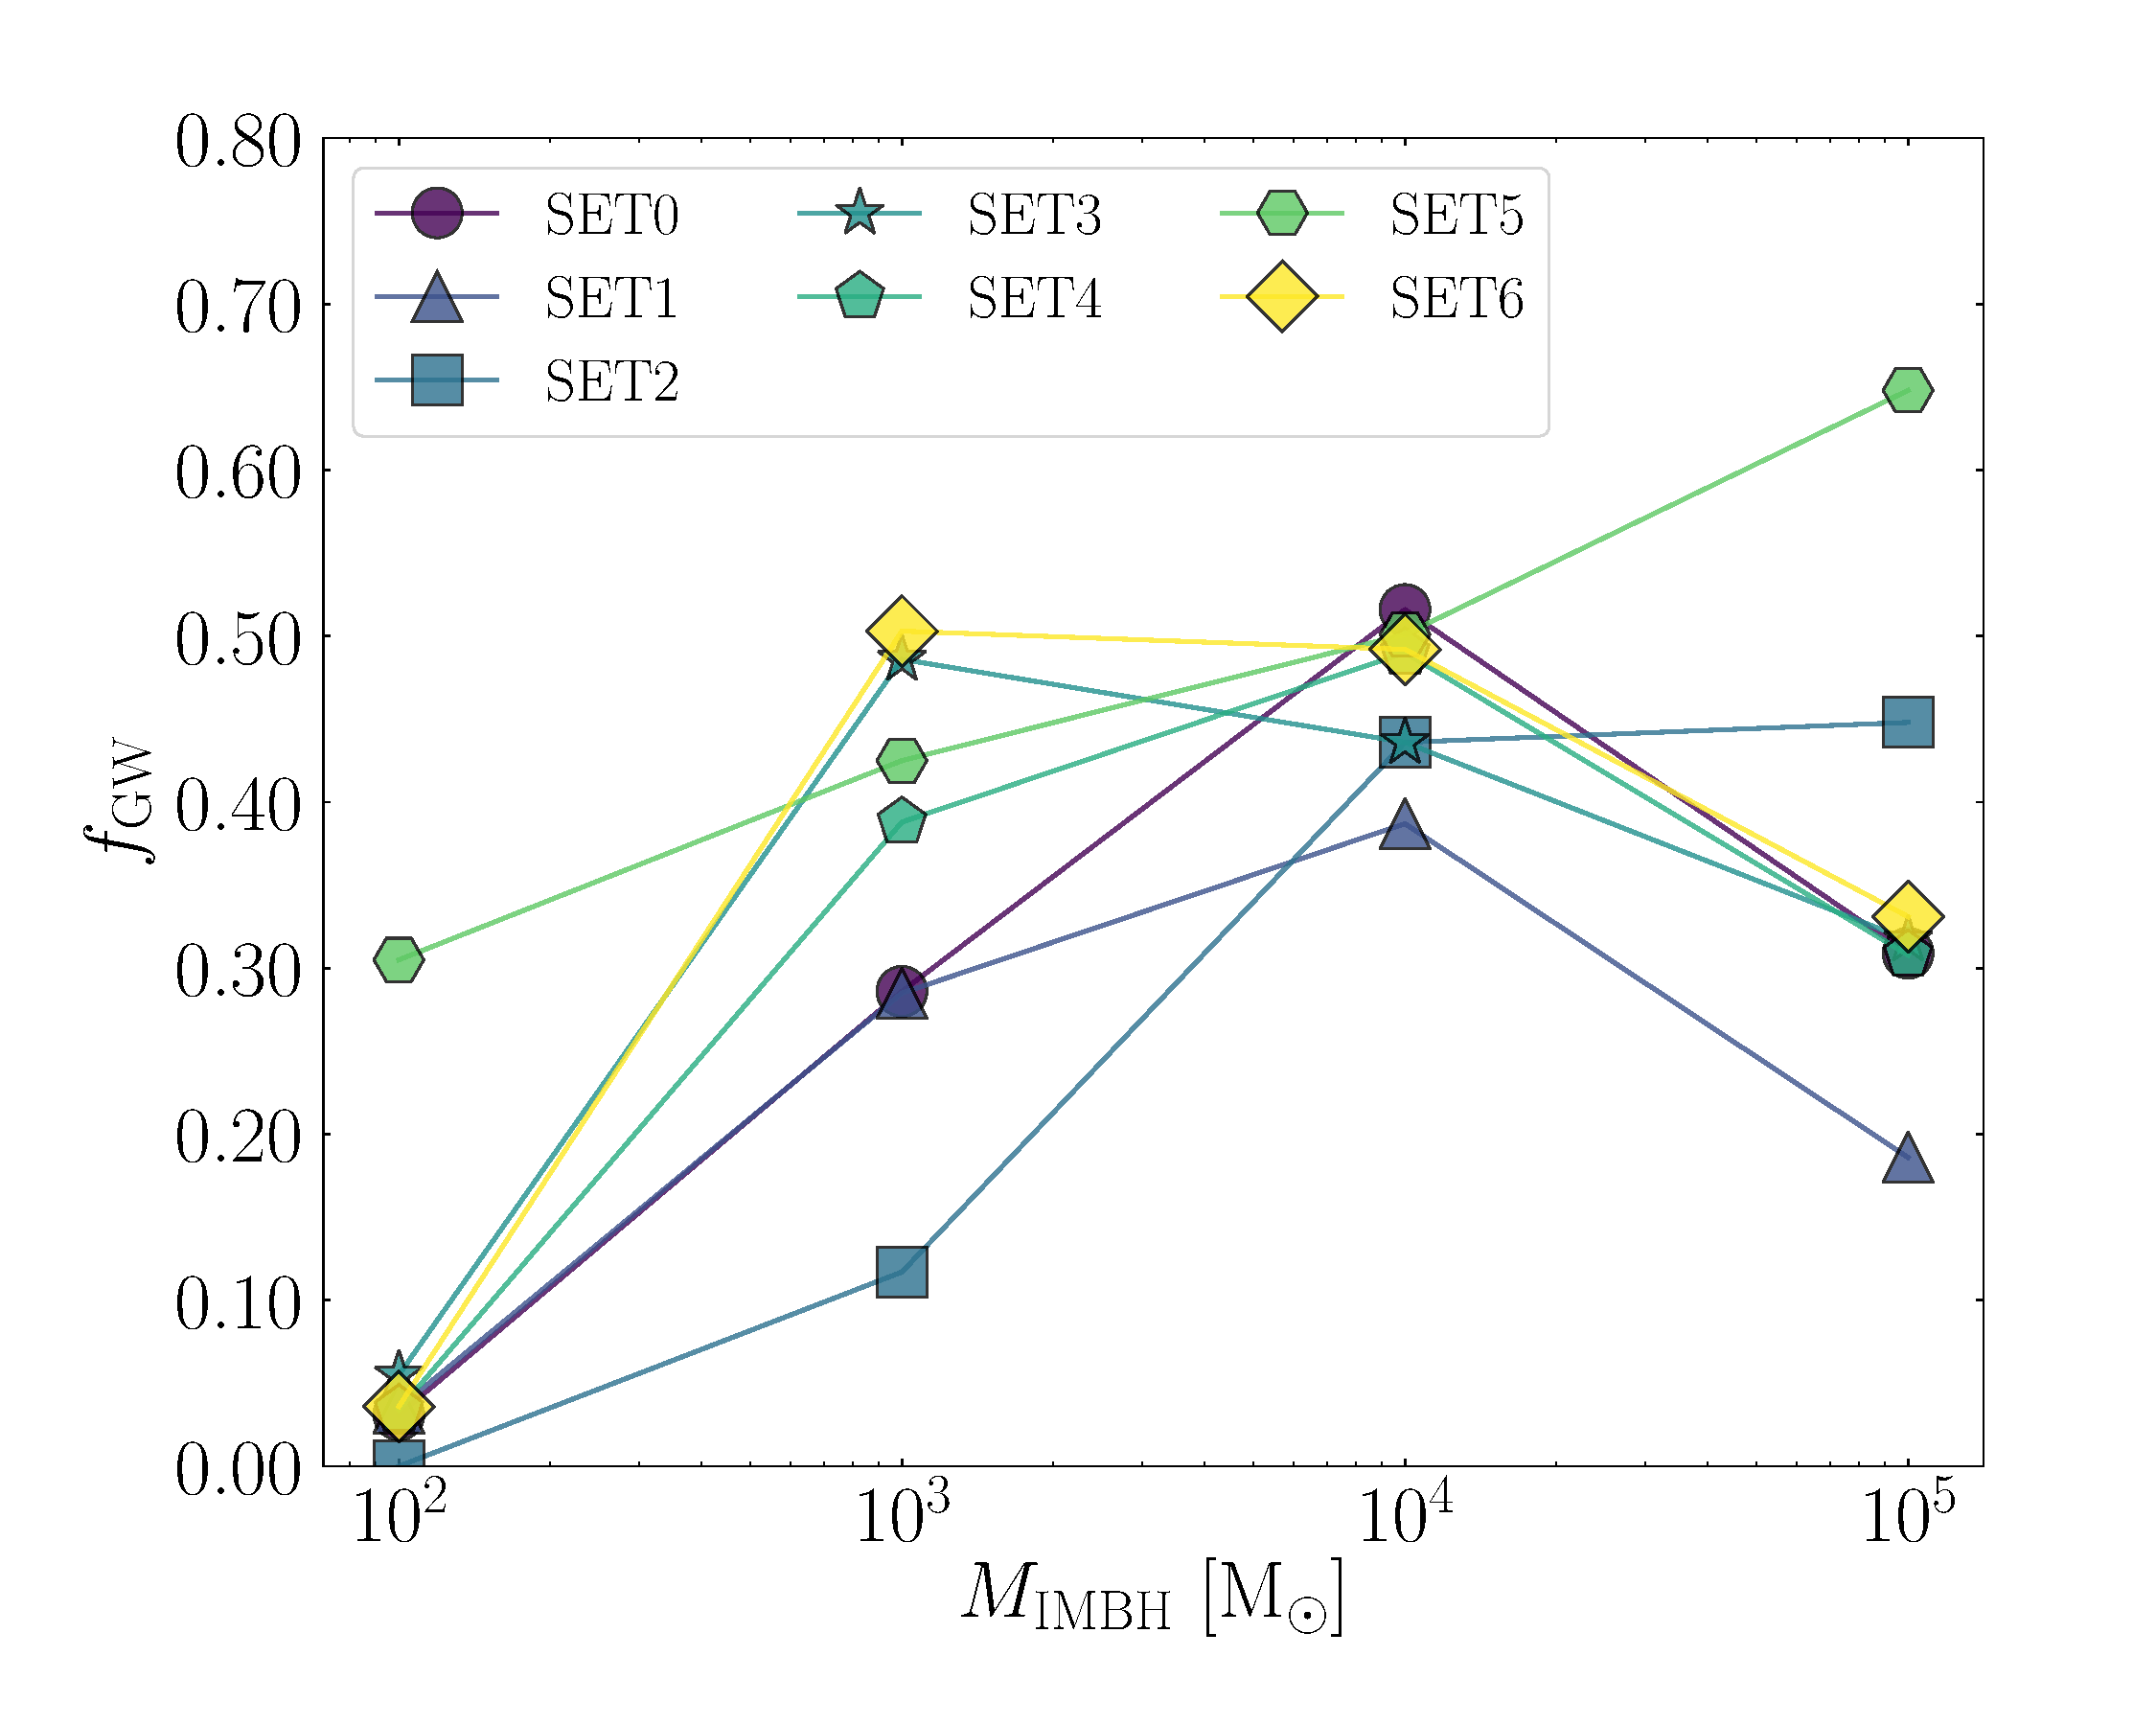
\includegraphics[width=\columnwidth]{mergerprob}
    \caption{IMRIs merger probability as a function of the IMBH mass for all models explored.}
	\label{fig:gwprob}
\end{figure}

While it is difficult to find a trend in the different models, in general our results suggest that the IMRI merger probability maximizes at IMBH masses $M_\ibh\sim 10^4\Ms$, while it is limited to a few percent in the case $M_{\ibh} = 100\Ms$. In the next section, we will exploit these results to infer the cosmological merger rate of IMRIs associated with different IMBH mass ranges and GW detectors.

Another important property that can be inferred from our models is the mass distribution ${\rm d}N/{\rm d}M_{\rm bh}$ of IMRI lighter companion, which is shown in Figure \ref{fig:f8} for models SET0-5 (different cluster density profiles and BH mass spectrum) and Figure \ref{fig:f8} for models SET0, 6 (different stellar metallicity). Comparing SET0, 1, and 3 -- which differ only in the cluster density profile but adopt the same BH mass spectrum \citep{spera17} -- it is apparent that the ${\rm d}N/{\rm d}M_{\rm bh}$ not depend on the environment, but rather on the BH mass spectrum adopted. In all three cases, the mass distribution shows a clearly bimodal distribution peaked at $\sim 7\Ms$ and $34\Ms$. The picture changes significantly if another BH mass spectrum is adopted. In the case of a power-law mass spectrum in the range $M_\bh = 3-30\Ms$ we find that ${\rm d}N/{\rm d}M_{\rm bh}$ declines sharply starting from $3\Ms$ and truncates at $> 25 \Ms$, whereas for a flat mass spectrum in the same range the trend turns out to be opposite, with the ${\rm d}N/{\rm d}M_{\rm bh}$ parameter increasing toward $25 \Ms$ and abruptly dropping beyond this value. Assuming smaller values for the initial semimajor axis (SET5) does not affect significantly the merging BH mass distribution, which in fact resembles that obtained for SET0-3. We explored whether the IMBH mass plays a role in shaping the merging BH mass distribution but, on average, we find that the overall distribution remains the same across all the range of $M_\ibh$ explored. As shown in Figure \ref{fig:mbhdist}, increasing the stellar metallicity to solar values (SET6) leads to IMRIs with a secondary component mass that remains below $25\Ms$. 

These results have two main implications. On the one hand, the IMRI secondary mass tells us something about the mass spectrum of BHs lurking around an IMBH. On the other hand, it provides clues about the IMBH formation process. In fact, if the IMBH formed during cluster's early life, we can expect that the BH mass spectrum isn't altered substantially by dynamics. However, if the IMBH develops after dynamical encounters shaped the BH reservoir -- for instance by causing the ejection of the most massive BHs -- we would expect that the IMRI secondary mass would preferentially attains lower values.

\begin{figure*}
\centering
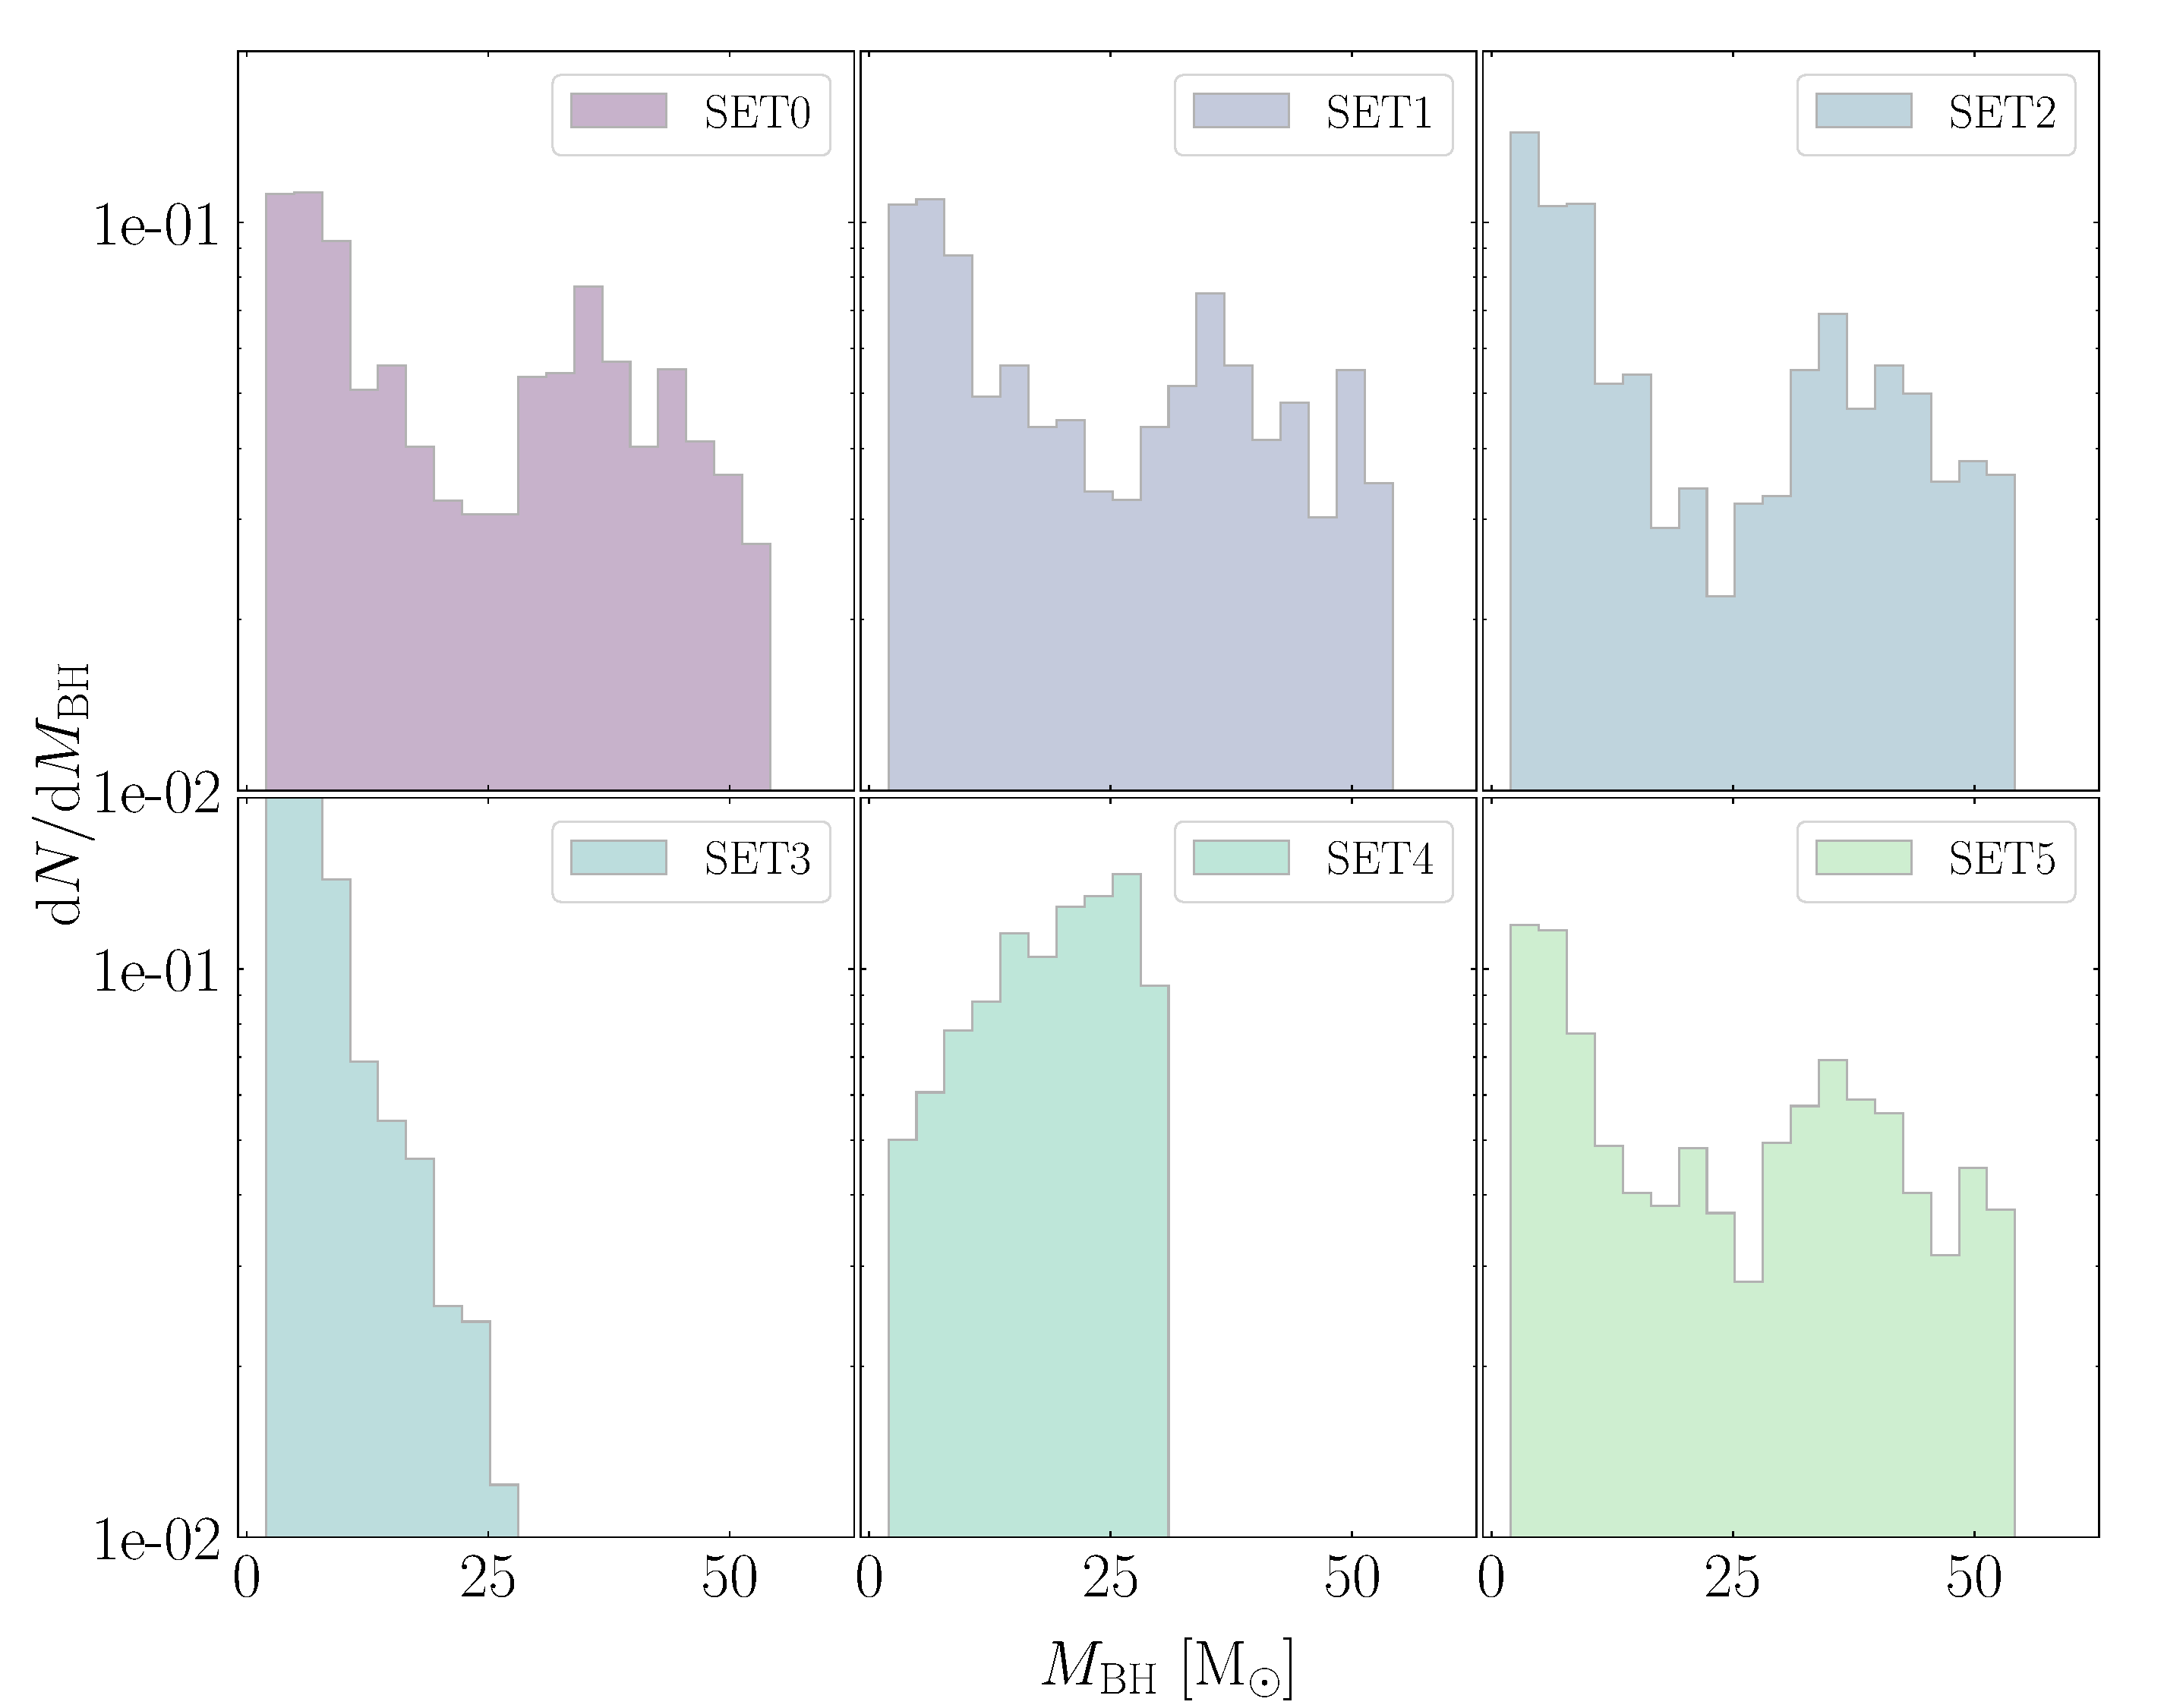
\includegraphics[width=0.8\textwidth]{massdis}\\
%\includegraphics[width=0.8\textwidth]{massdisD}\\
    \caption{%Top panel: 
    Mass distribution of the IMRI secondary for SET0 to 5. Each color corresponds to a different set to facilitate the comparison between different panels and figures. 
    %Bottom panel: the same as above, but differentiating for different IMBH masses: $10^2\Ms$ (straight line), $10^3\Ms$ (dashed line), $10^4\Ms$ (dashed dotted line), $10^5\Ms$ (dotted line) as indicated in the legend. Each color corresponds to a different set to facilitate the comparison between the upper and lower panels.
    }
	\label{fig:f8}
\end{figure*}

\begin{figure}
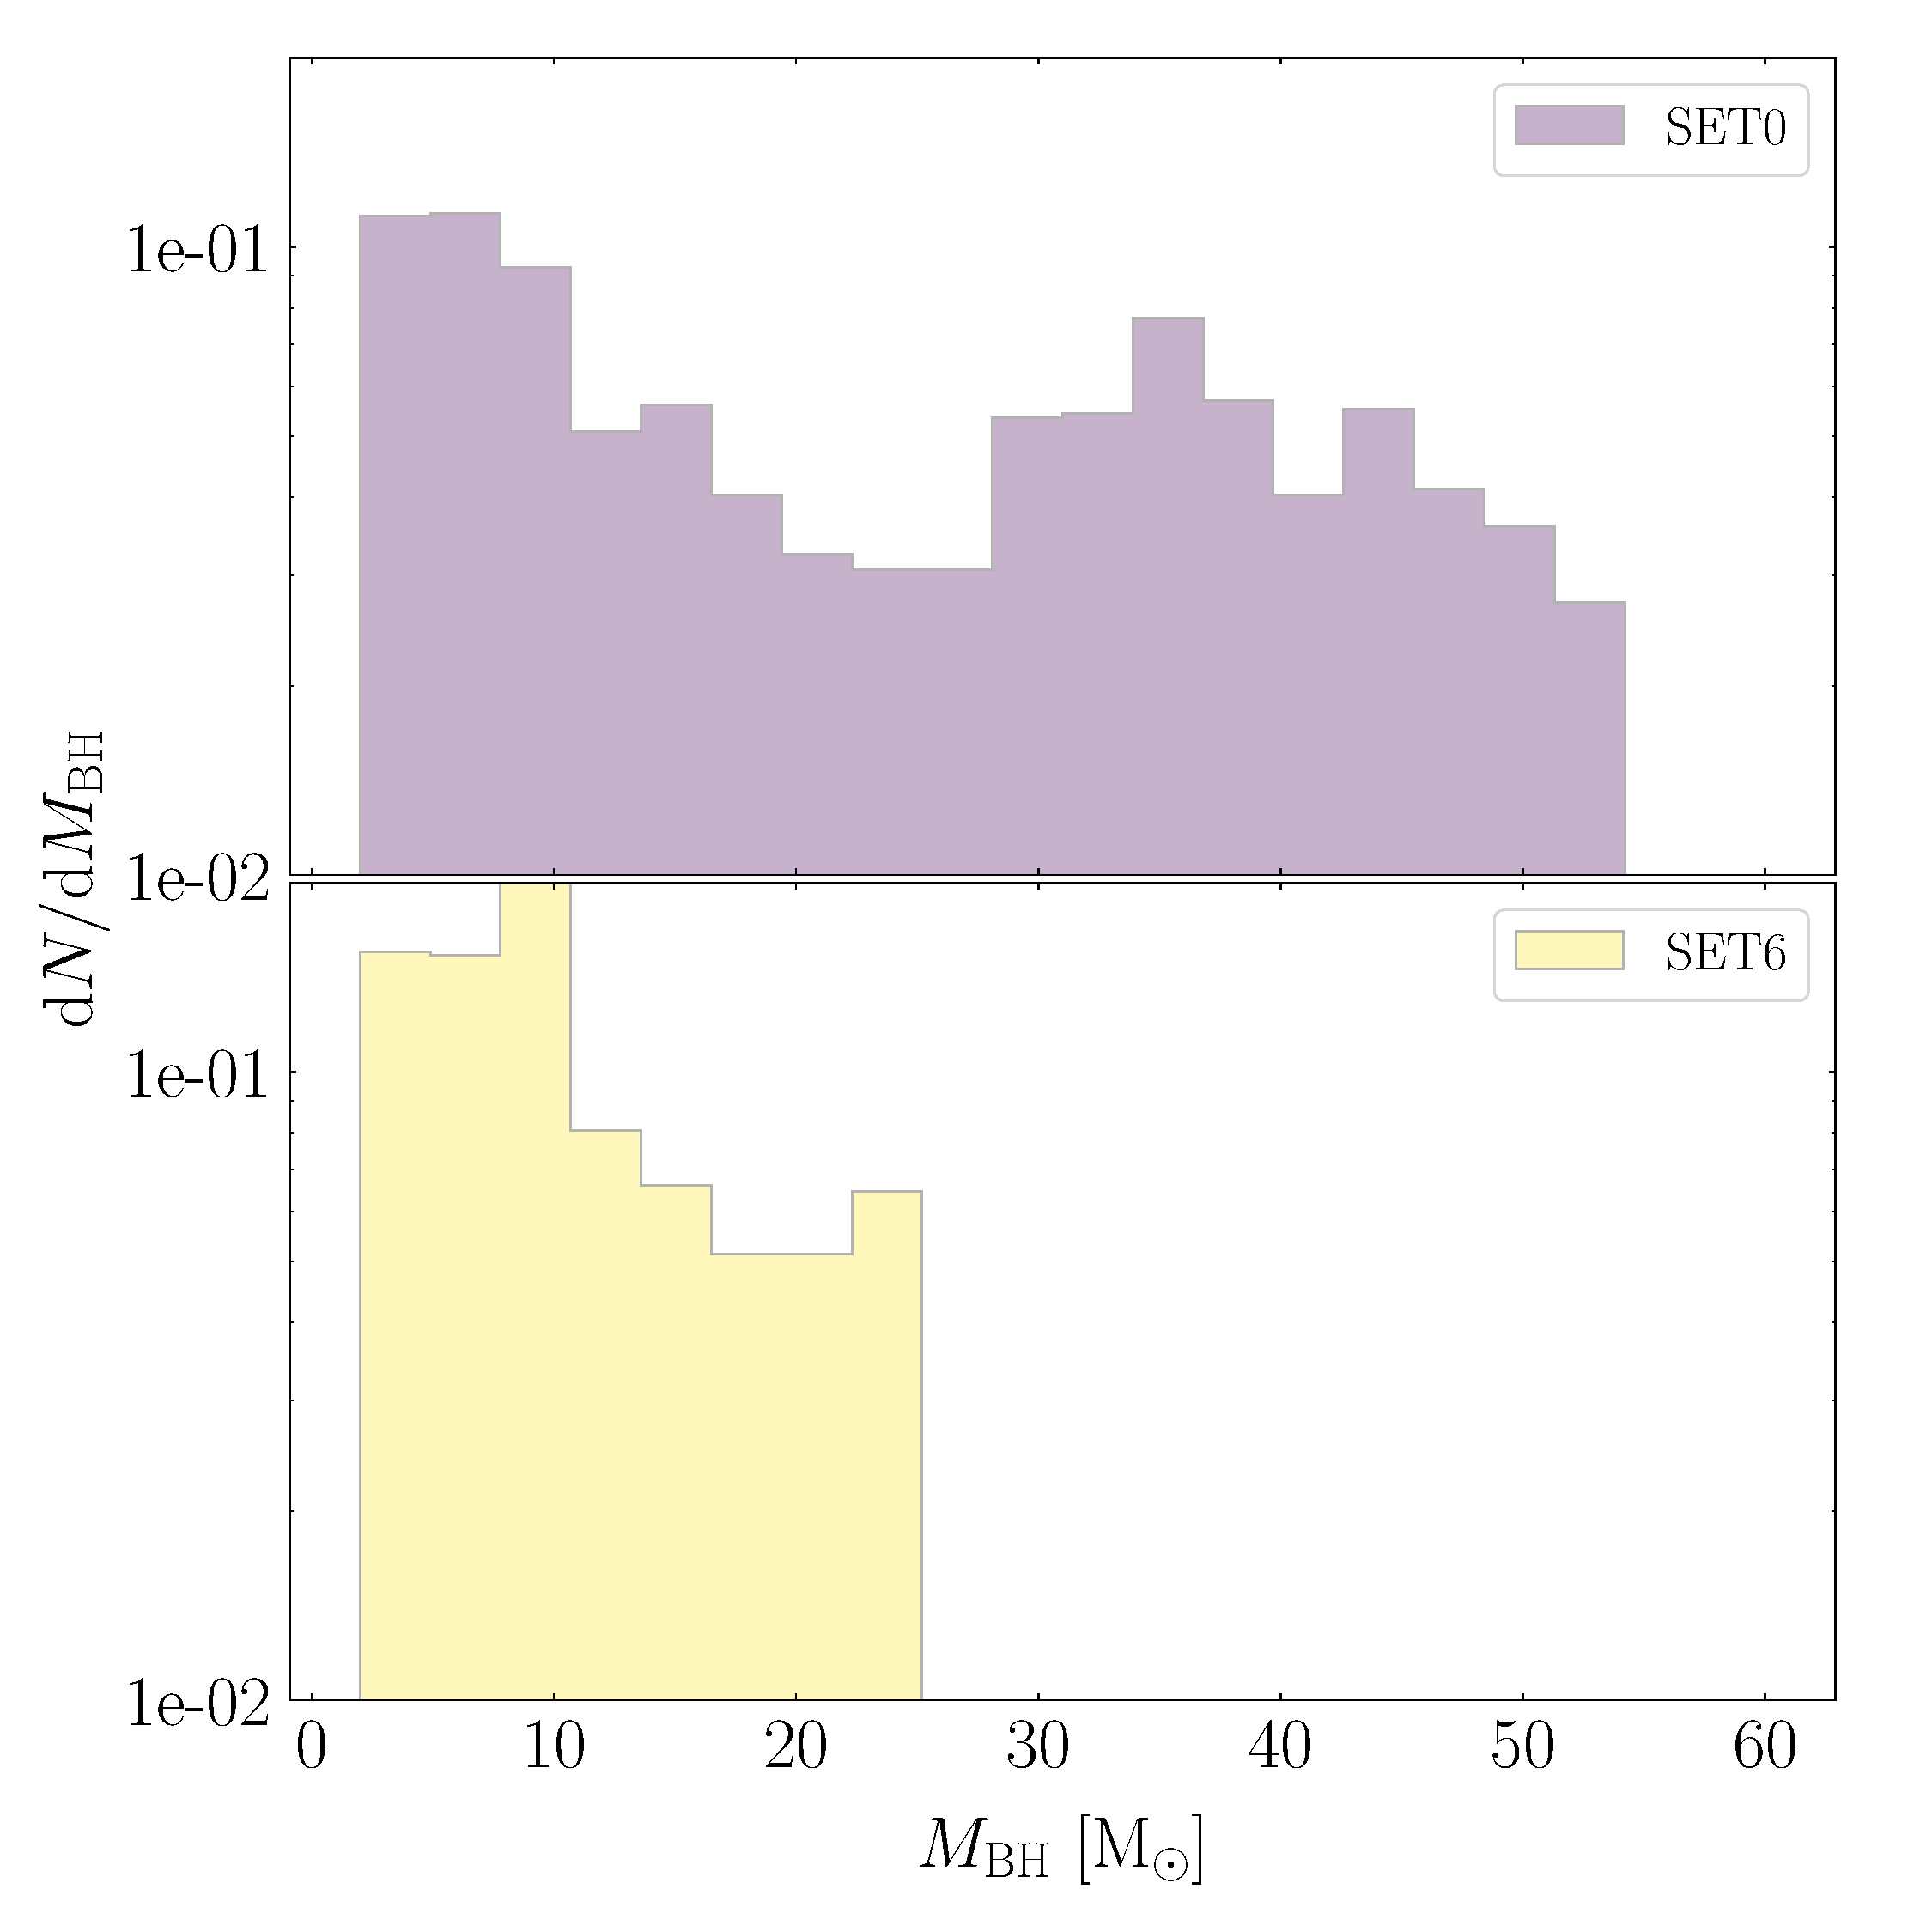
\includegraphics[width=\columnwidth]{massdis06}
    \caption{Mass distribution of the IMRI secondary for SET0 and SET6, which rely on the same set of assumption except for the initial metallicity: $Z = 0.0002$ (SET0), and $Z = 0.02$ (SET6).}
	\label{fig:mbhdist}
\end{figure}


The distribution of merger times $t_\gw$ seems to be independent on the set of adopted initial conditions. As suggested by Figure \ref{fig:f10}, which shows the cumulative $t_\gw$ for all models, around $50\%$ of mergers have $t_{\gw} < 10^6 - 10^7$ yr, with the exception of SET2 for which  $t_{\gw} \sim 10^8$ yr. 


\begin{figure}
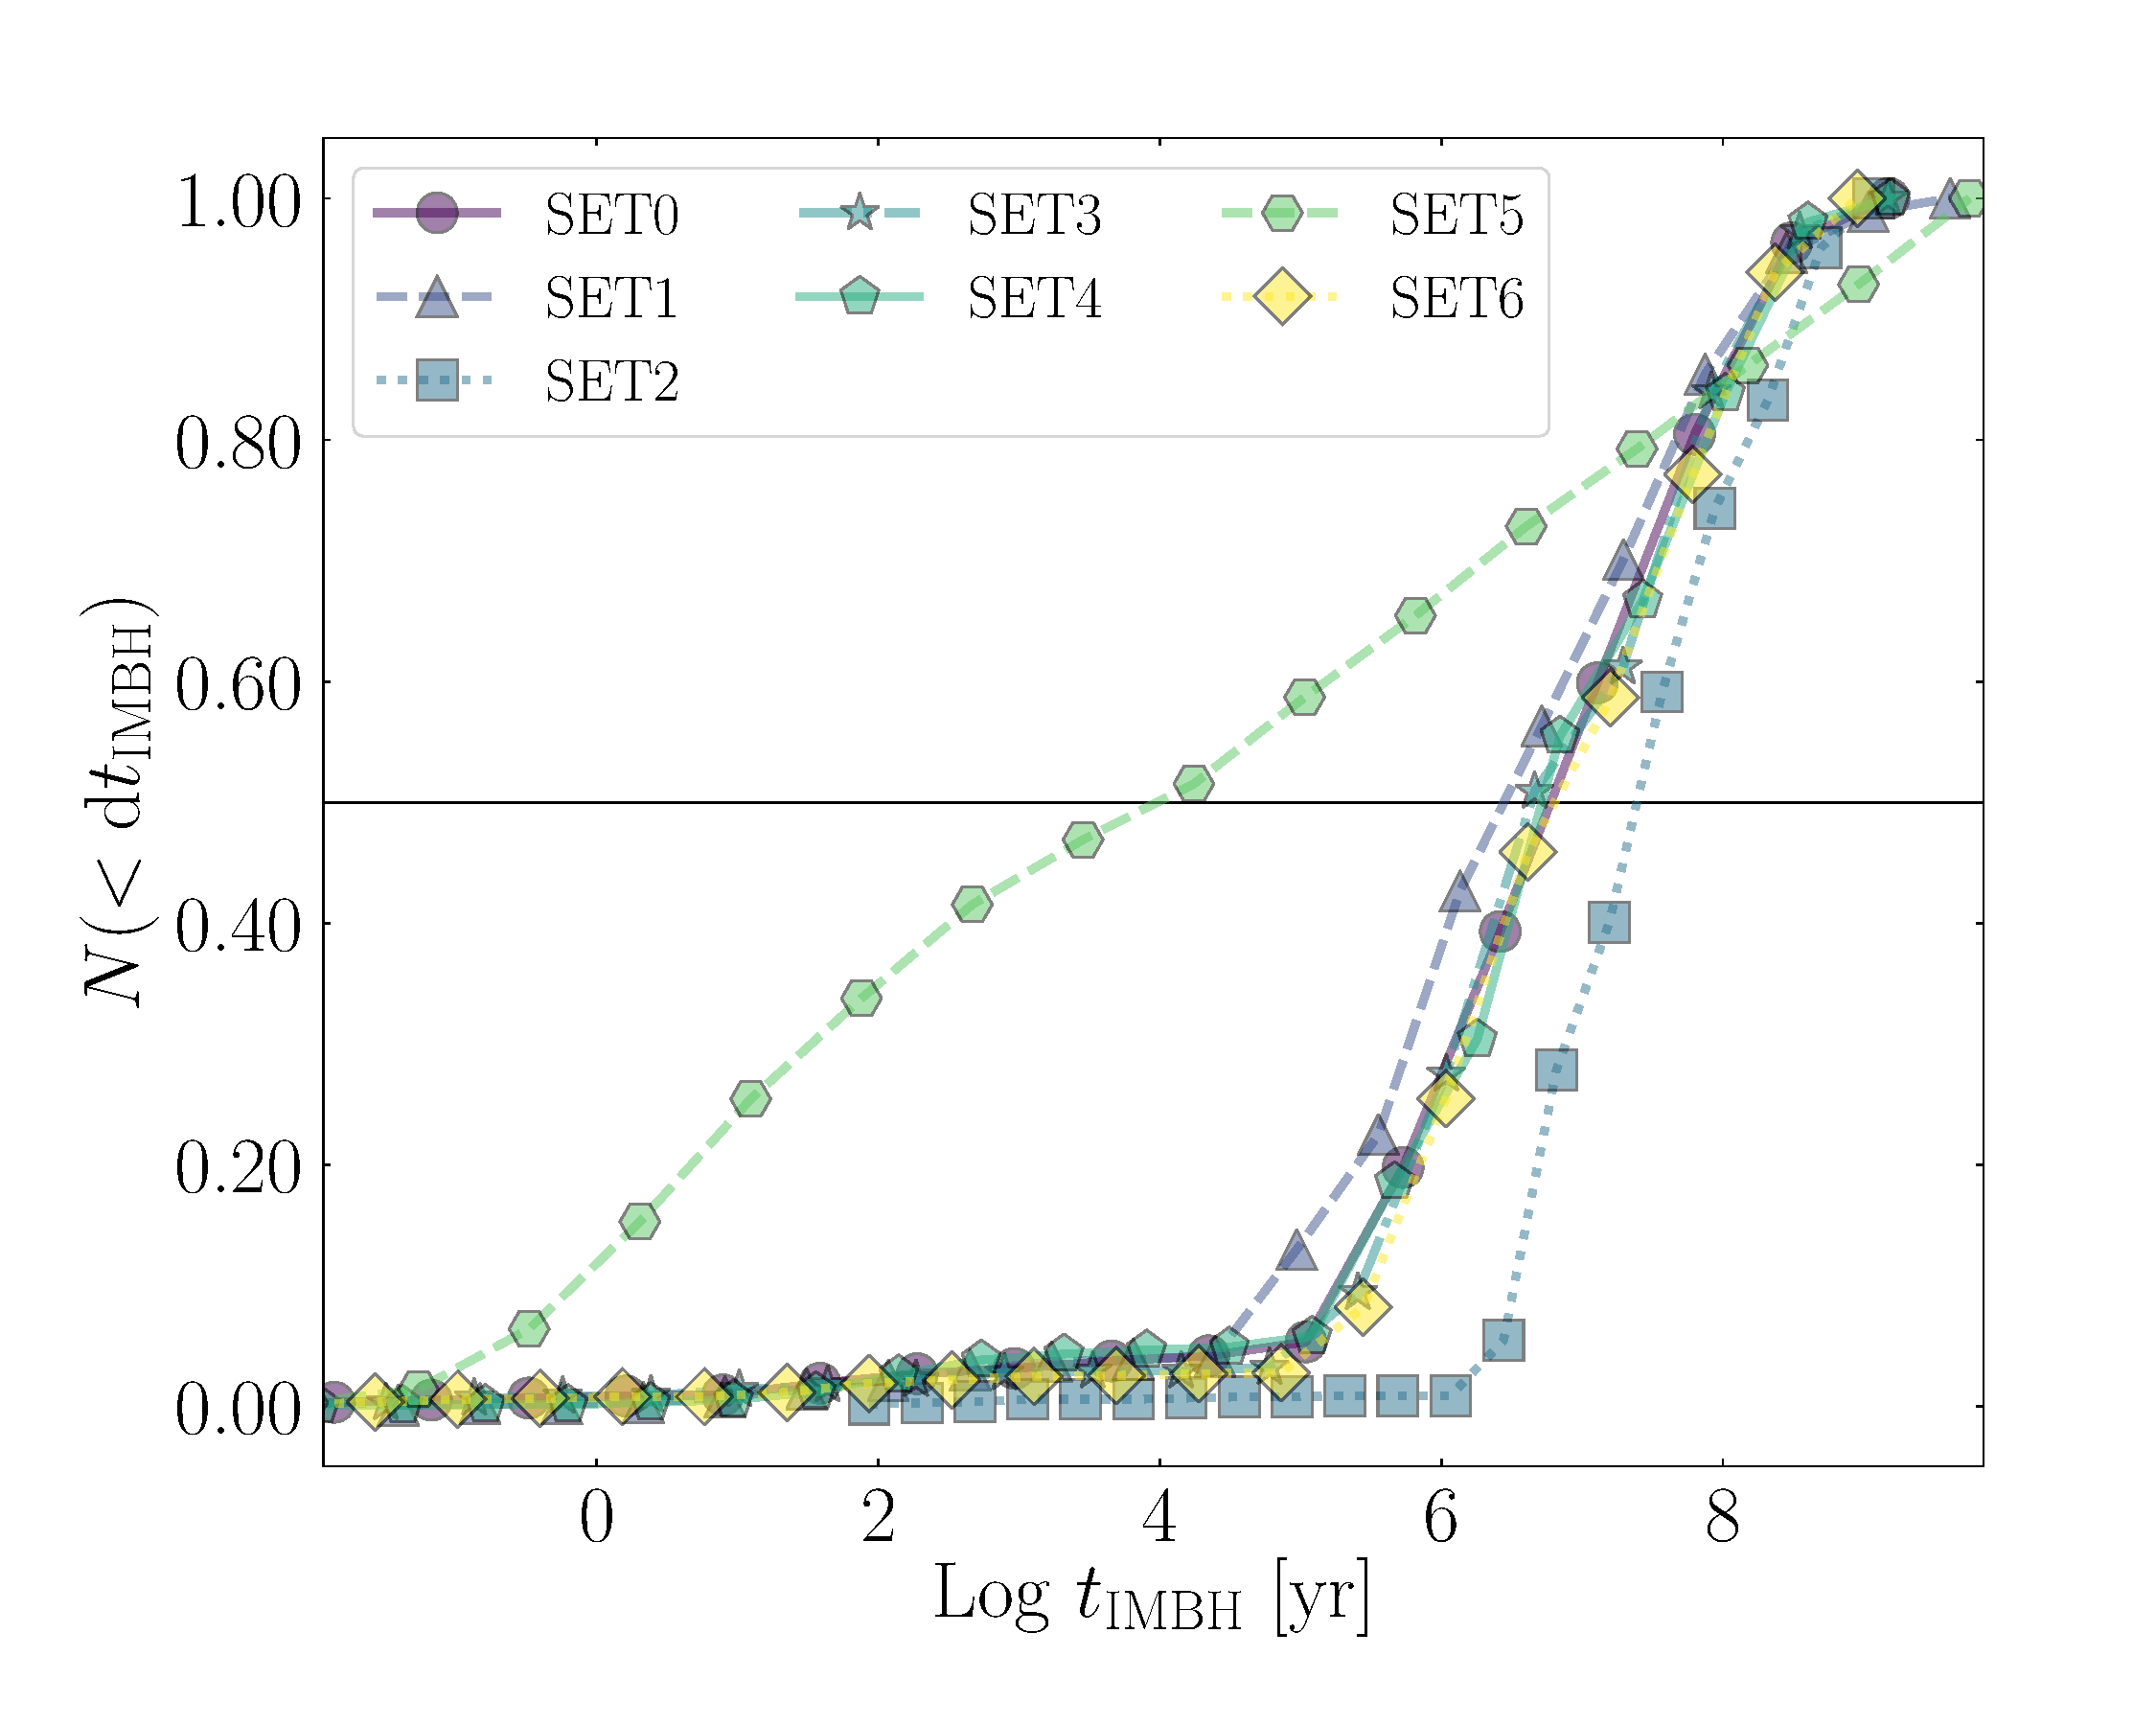
\includegraphics[width=\columnwidth]{time}
    \caption{Distribution of IMRI merging times calculated for all mergers in all the models explored. Different colors and symbols correspond to a different model SET as indicated in the legend.}
	\label{fig:f10a}
\end{figure}



}


\subsection{IMBH survival in dense star clusters}
{\bf
Promptly after a merger event, the anysotropic emission of GWs can impart a recoil kick to the merger product, depending on the mass and spin of the two merging objects \citep{campanelli07,gonzalez07,lousto08,lousto12}. Depending on the kick amplitude, the recoil can kick out the IMBH from the cluster \citep[e.g.][]{bockelmann08}, leading it to wander forever outside the cluster. In fact, for low-velocity dispersion ($5$ km/s) star clusters the probability to retain a BH with mass $m_\bh> 100 \Ms$ after 1-2 consecutive mergers is rather low, $1-5\%$ \citep{arca20}. To place constraints on the IMBH retention probability, we create a catalogue of IMRI mergers proceeding on a step-by-step basis as follows: 
\begin{enumerate}
\item we divide the IMBH mass range -- $M_\ibh = 10^2-5\times 10^5\Ms$ -- in 15 values evenly distributed in logarithmic values;
\item for each IMBH mass, we create a sample of 100 stellar BHs with masses evenly drawn in the $M_\bh = 3.5-80 \Ms$ range;
\item we associate to the IMBH and BH a spin randomly drawn between 0-1;
\item we use \cite{jimenez17} numerical relativity fitting formulae to calculate the IMRI merger remnant mass $M_r$, spin $S_r$, and recoil velocity $v_r$, following the procedure depicted in \cite{arca20}.
\end{enumerate}
For each $M_\ibh -m_\bh$ pair, we repeat steps 3 and 4 100 times and, for each of them, we compare the recoil velocity with the escape velocity from the cluster centre, which we set to $\sigma = 5$ or $50$ km/s. 

The result of this procedure is described in Figure \ref{fig:f11}, which shows the percentage of models for which $v_r < \sigma$. In the case of 
a ''normal'' cluster ($\sigma = 5$ km/s), we find that an IMBH with mass $M_\ibh < 200 \Ms$ gets ejected whenever the merging companion has a mass $m_\bh \geq 10 \Ms$. Even for heavier IMBHs, e.g. $M_\ibh = 1000\Ms$, the retention probability rapidly drops below $50\%$  if the companion mass exceeds $M_\bh > 20\Ms$. Only for quite heavy IMBHs ($M_\ibh \sim 10^4\Ms$) the retention probability attains values $>80\%$ regardless the secondary BH mass. In the case of a denser cluster ($\sigma=50$ km/s), we find that a moderate IMBH ($M_\ibh \sim 200-300 \Ms$) have a $50\%$ retention probability if $m_\bh < 30\Ms$, while for $M_\ibh = 1000\Ms$ the BH mass threshold to ensure a $50\%$ retaining probability increases to $m_\bh = 70\Ms$.

Therefore, localizing an IMBH in the centre of a star cluster and measuring its mass would enable us to get insights on its evolution. For instance, the presence of an IMBH with mass $>10^3\Ms$, even in dense clusters, would suggest that the IMBH growth process might be dominated  by matter accretion from disrupted star rather than by mergers with BHs heavier than $30-50\Ms$.
}

\begin{figure}
\centering
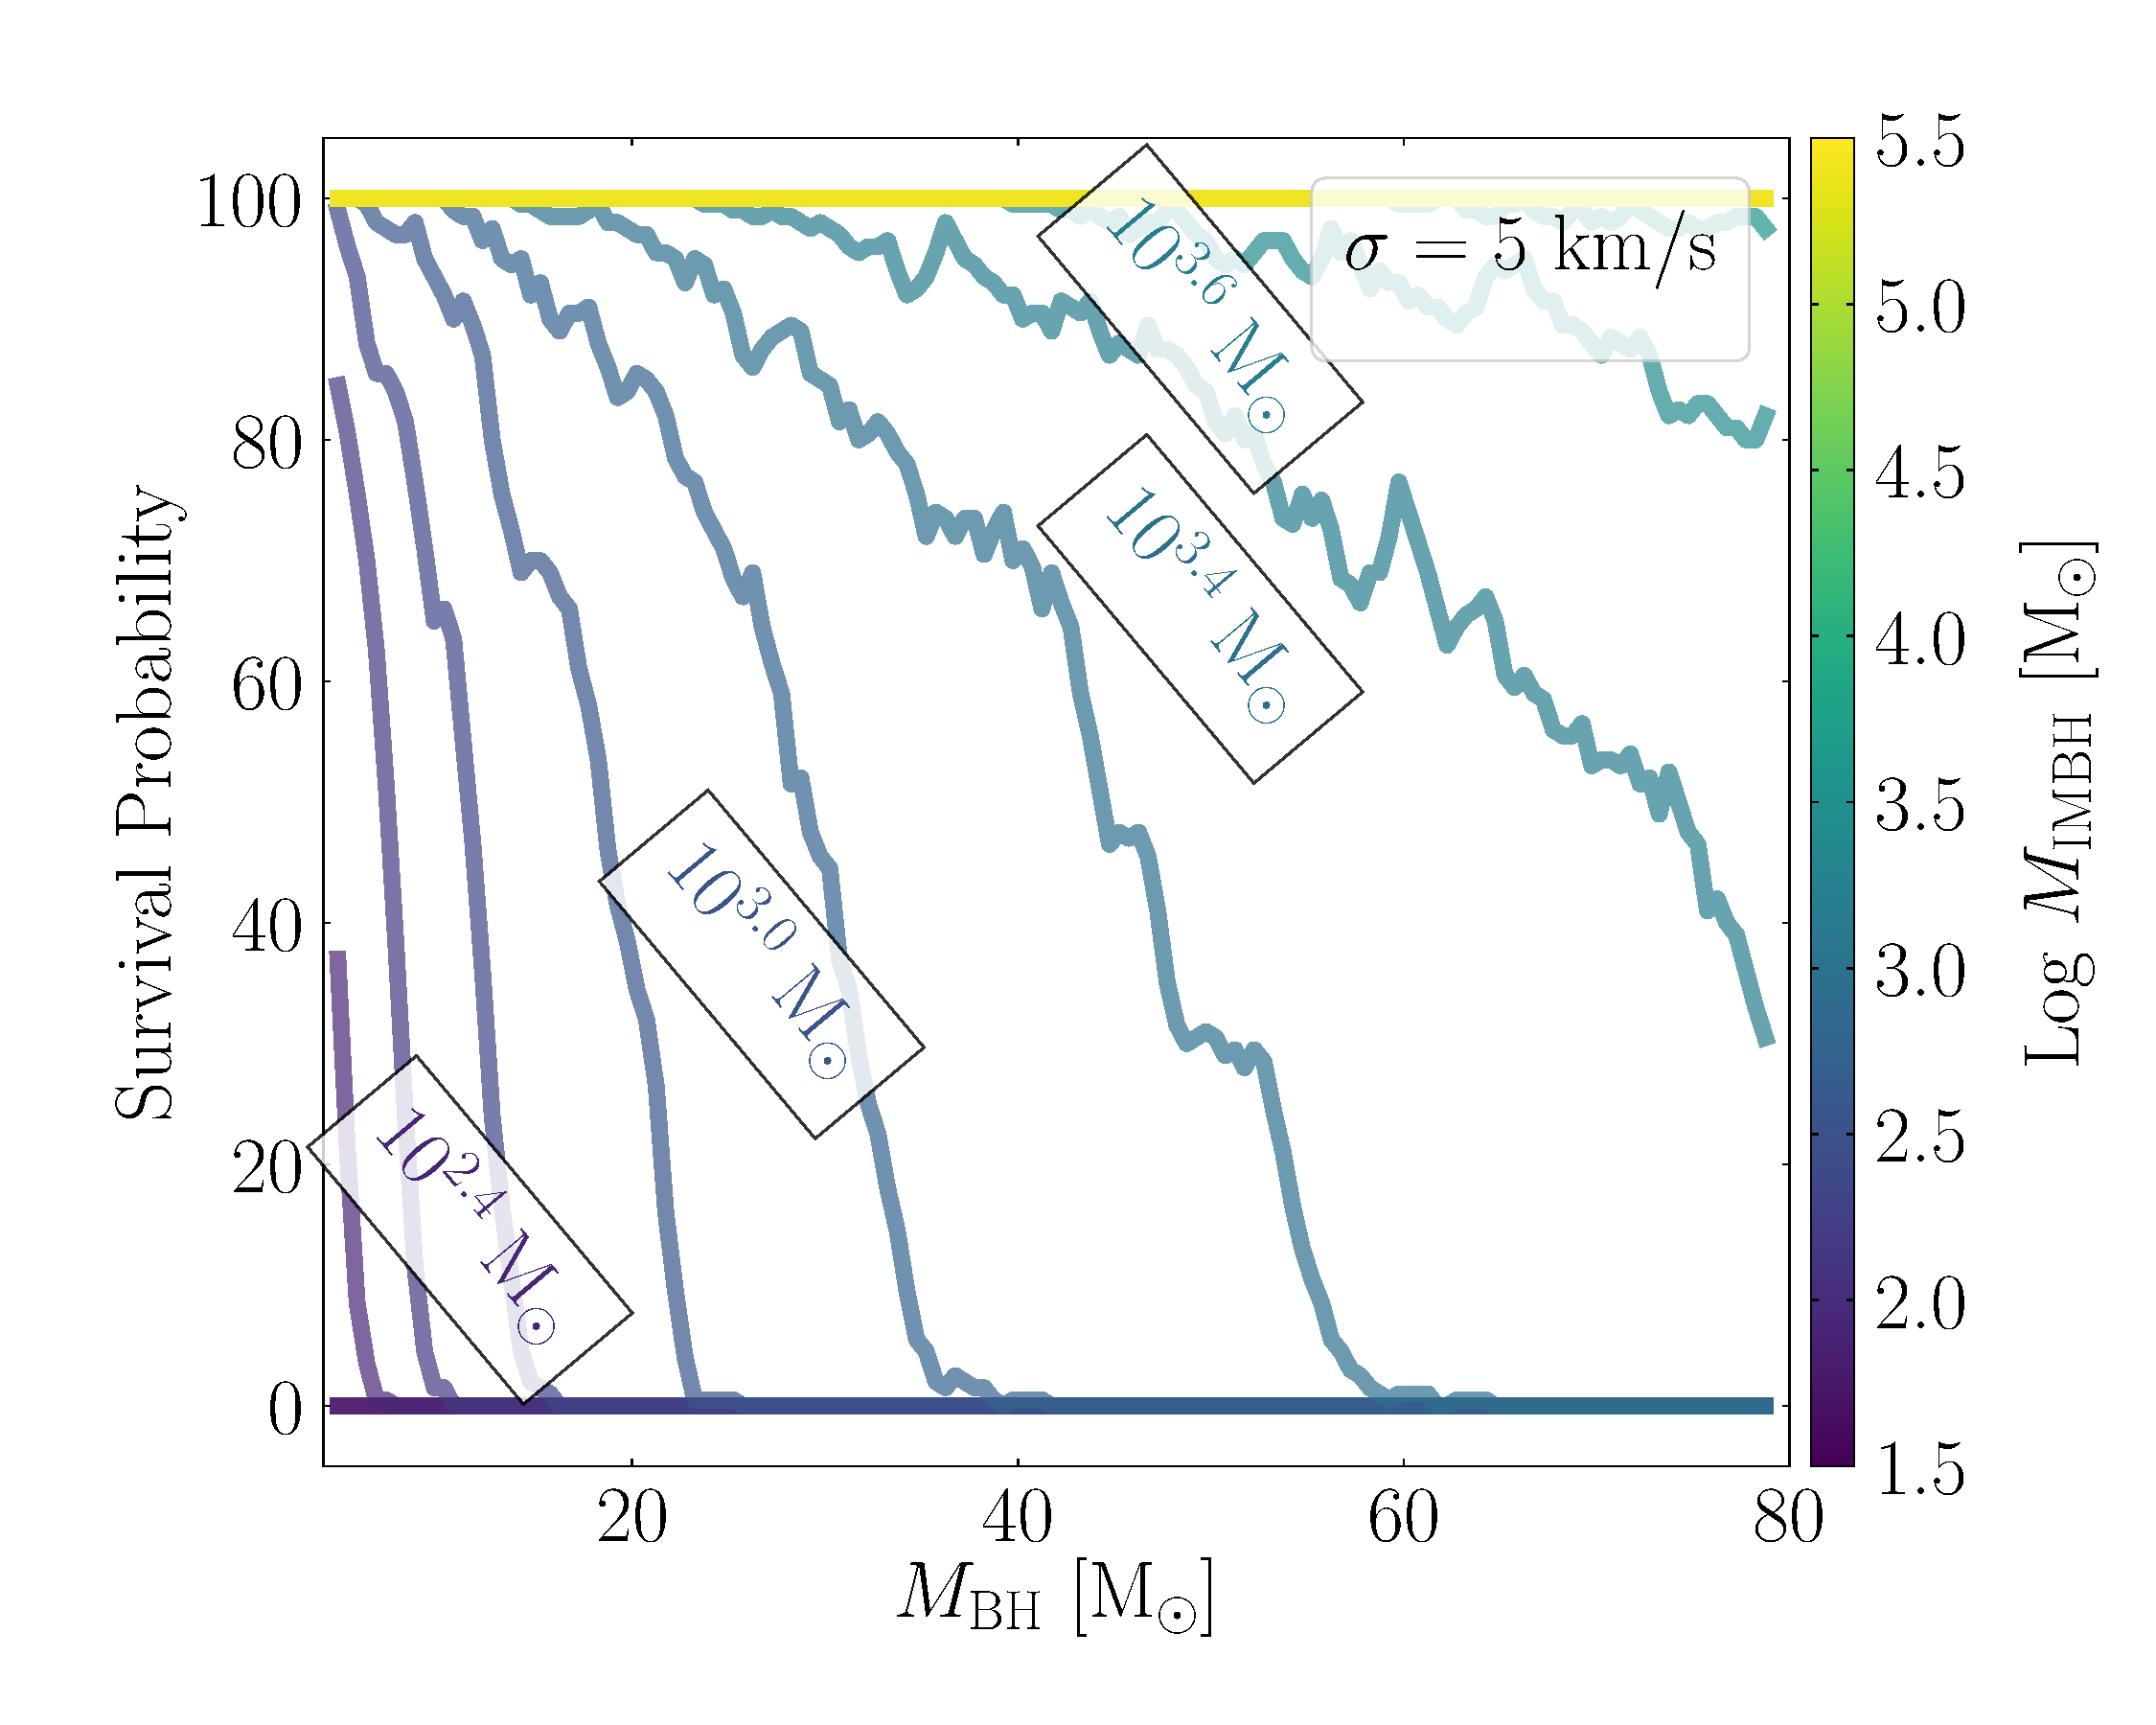
\includegraphics[width=\columnwidth]{survival}
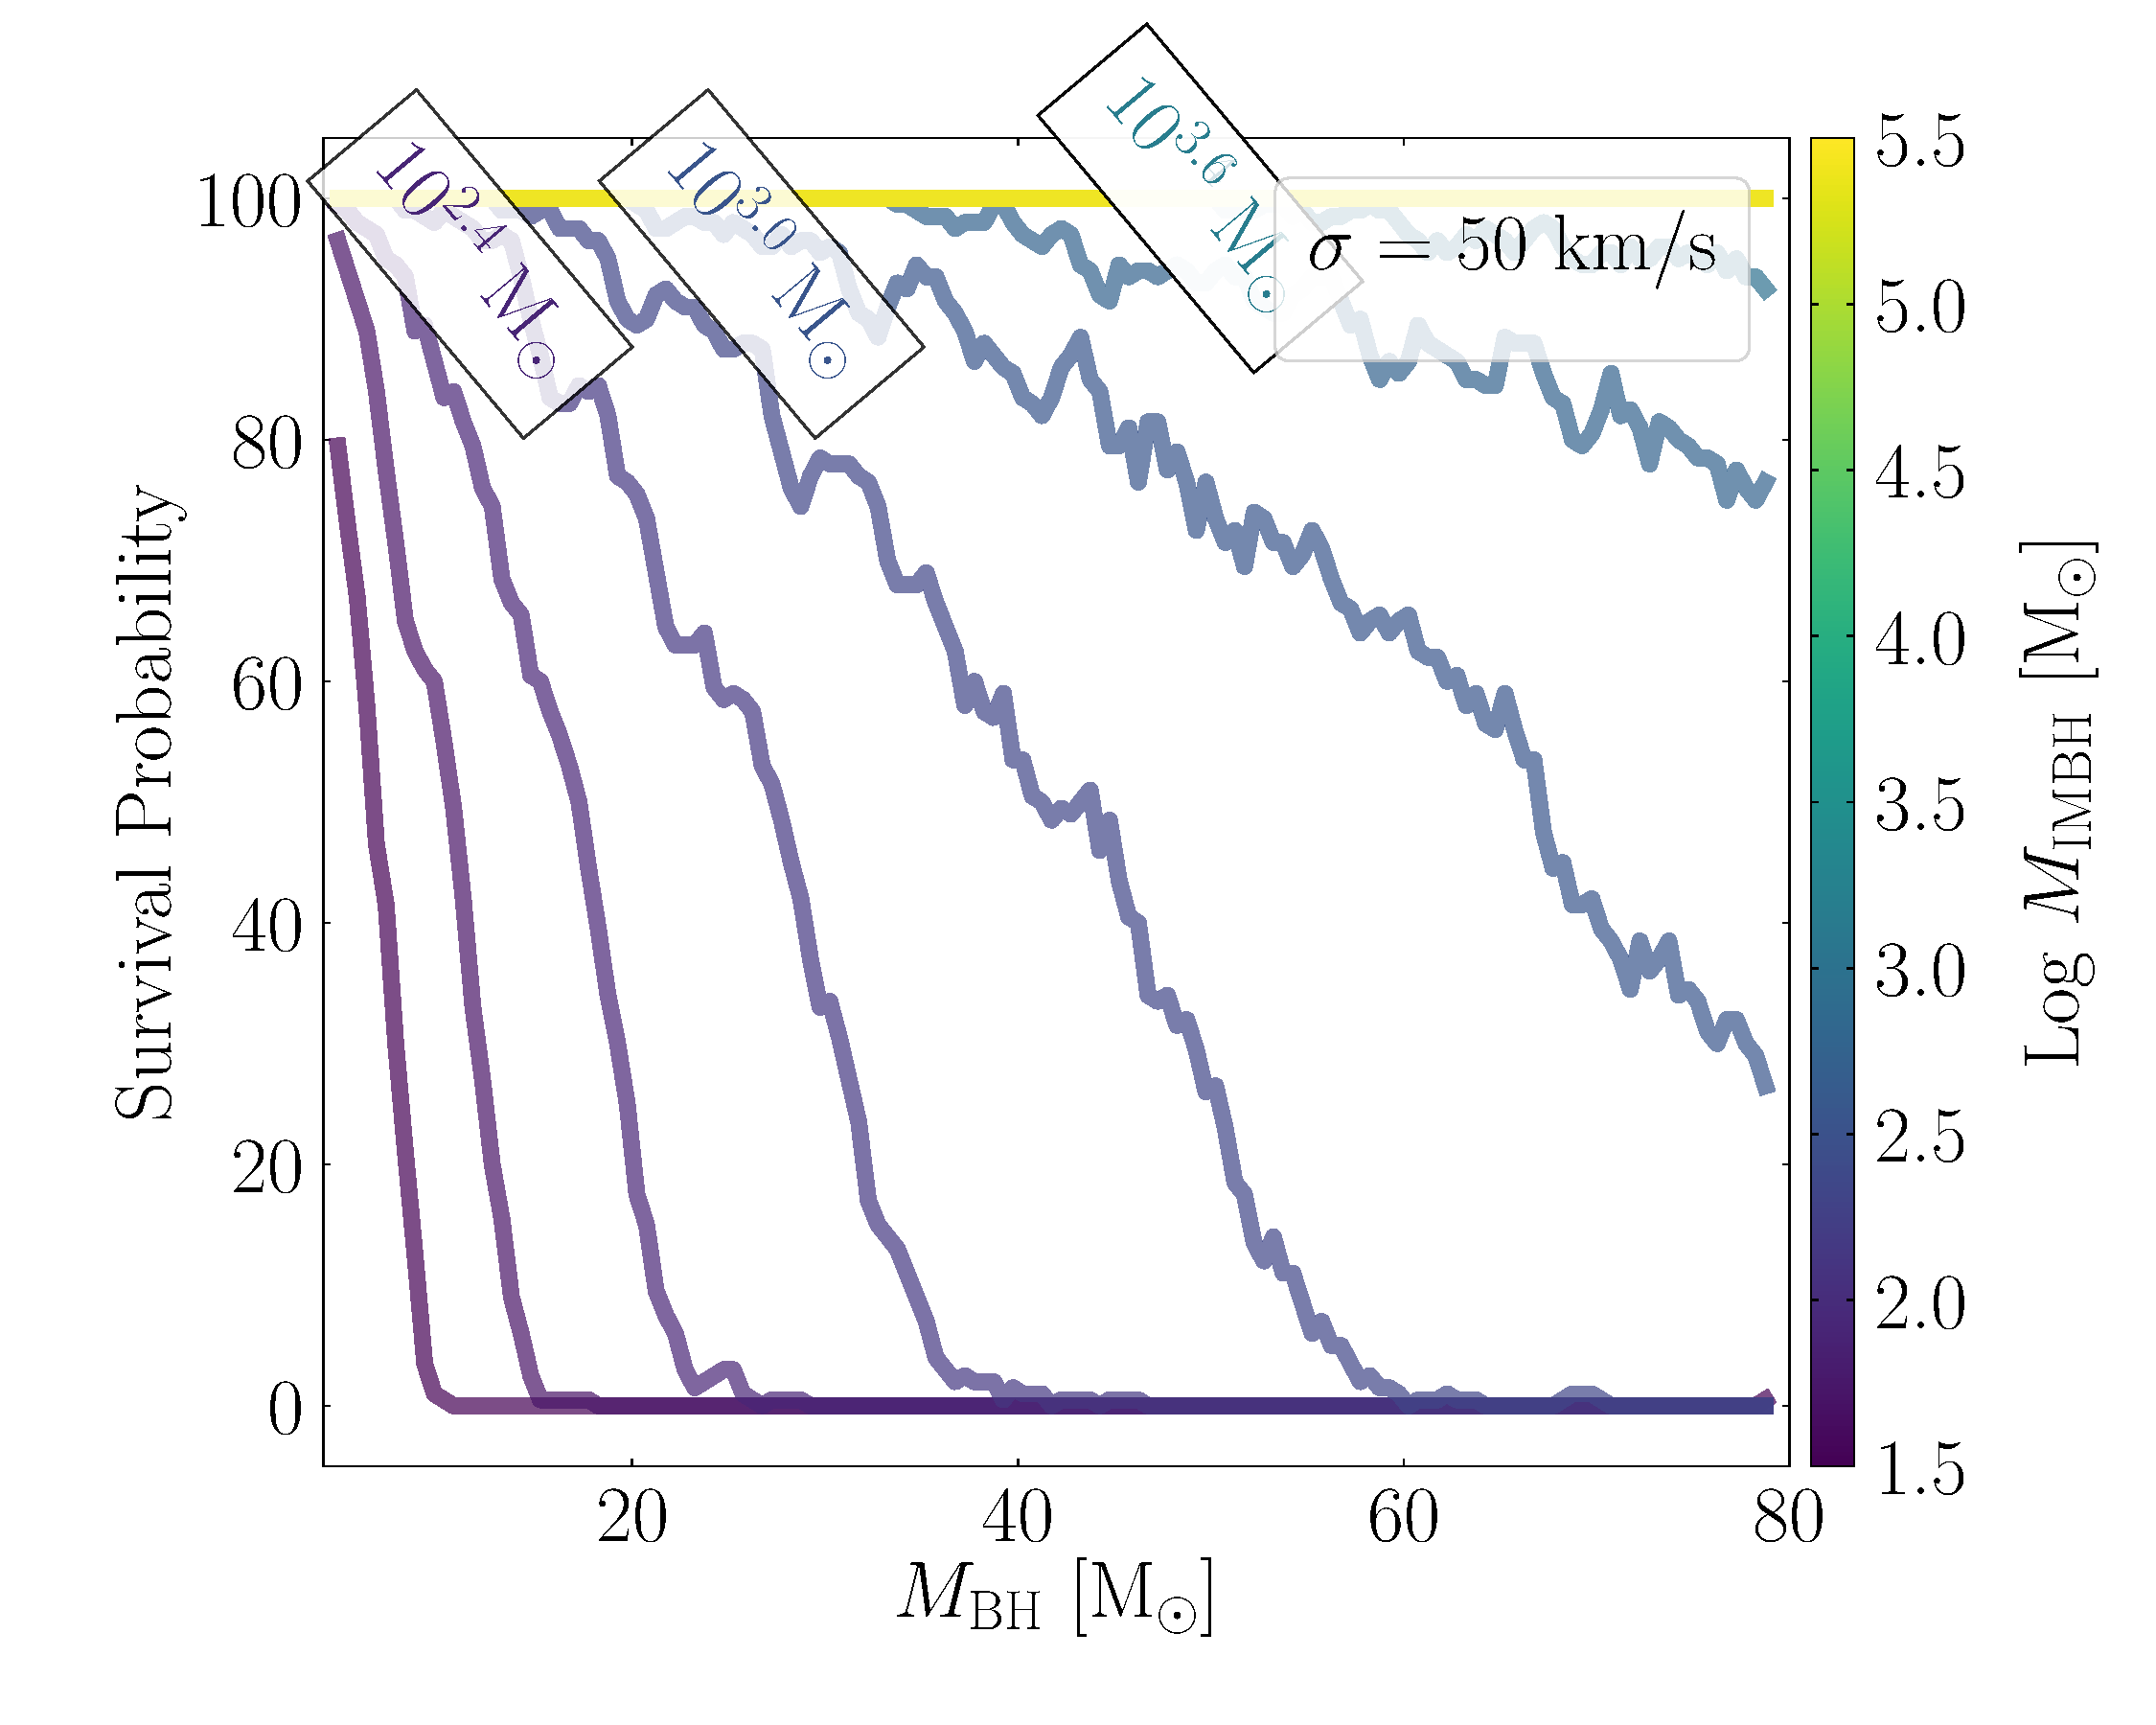
\includegraphics[width=\columnwidth]{survival50}
\caption{Top panel: IMBH retention probability as a function of the merging BH mass for different values of the IMBH mass, identified by the color-coding, assuming for the star cluster an escape velocity of $\sigma = 5$ km/s. Bottom panel: same as above, but for an escape velocity of $\sigma = 50$ km/s.}
\label{fig:survival}
\end{figure}


\subsection{IMBHs spin evolution}
{\bf 
Since an IMBH-BH merger cause an inevitable variation of the IMBH spin, this quantity might be useful to get insights on the IMBH evolution.
To support this idea, we create a sample of IMBH-BH mergers as follows. We select an IMBH with mass of either $M_\ibh = 10^2 - 10^3 - 10^4 - 10^5$ and spin $S_\ibh = 0.1 - 0.5 - 0.9$ and we merge it with a stellar BH with mass in the range $3 - 60 \Ms$ drawn randomly and spin drawn accordingly to a Gaussian distribution with mean $S_\bh = 0.7$ -- i.e. the average value inferred from LIGO O1+O2 observations -- and dispersion 0.1.

Figure \ref{fig:f11a} shows the value of the remnant IMBH spin as a function of the IMRI mass ratio. 

We see that as long as the mass ratio remains below $10^{-2}$ -- which implies an $M_\ibh > 10^4 \Ms$ -- the IMBH spin is not affected by the merger. However, for IMRIs with a mass ratio > 0.01, the remnant IMBH spin can change significantly. For mass ratios in the range $q = 0.01-0.1$ the spin variation is $\sim \pm 0.1$ with respect to the initial value, whereas at larger mass ratio values we see that the spin tend to move toward values close to the average value assumed for the BH spin distribution, being the remnant spin $S_r \sim 0.8\pm 0.2$.
The peculiar dependence between the remnant spin and the IMRI mass ratio has important consequences for the IMBH evolution. One the one hand, if the IMBH formed from the collapse of a gaseous cloud or a very massive star born out of stellar collisions and reach masses $\gtrsim 10^4\Ms$, measuring its spin in a IMRI merger would provide us with information on the processes that regulated the IMBH very formation. On the other hand,
if the IMBH formed via multiple mergers in a stellar environment rich in BHs, the remnant spin can provide clues on the spin distribution of the underlying population of stellar BHs.

To further investigate this point, we explore the effects of a series of subsequent mergers on the IMBH final spin in the case of 
an IMBH mass value  that ensure a retention probability of at least $50\%$ in an IMRI merger event involving a BH smaller than $40\Ms$.
From Figure \ref{fig:survival} and Figure\ref{fig:f11a} we thus select $M_\ibh = 10^3\Ms$, which satisfies the requirement above, and set its spin to either $S_\ibh = 0.1-0.5-0.9$. For each spin value, we model ten consecutive mergers with stellar BHs with masses $3-60\Ms$ and spin drawn from a Gaussian distribution with average $S_\bh = 0.5$ and dispersion 0.1. This sequence represents an {\it IMBH merger tree}. For each value of the spin we create 100 merger trees and calculate the IMBH spin evolution as shown in Figure \ref{fig:f11b}.
We note that all models tend to converge toward the mean value of the adopted spin distribution for stellar BHs, thus suggesting that it could be possible to link the IMBH spin with the overall spin distribution of stellar BHs inhabiting the star cluster. Infact, complementing a measure of the IMBH spin with the spin distribution inferred from stellar BH mergers observed as GW sources can help in unravelling the IMBH evolution, whether it was driven by mergers with compact objects or by stellar feeding.
}

\begin{figure}
\centering
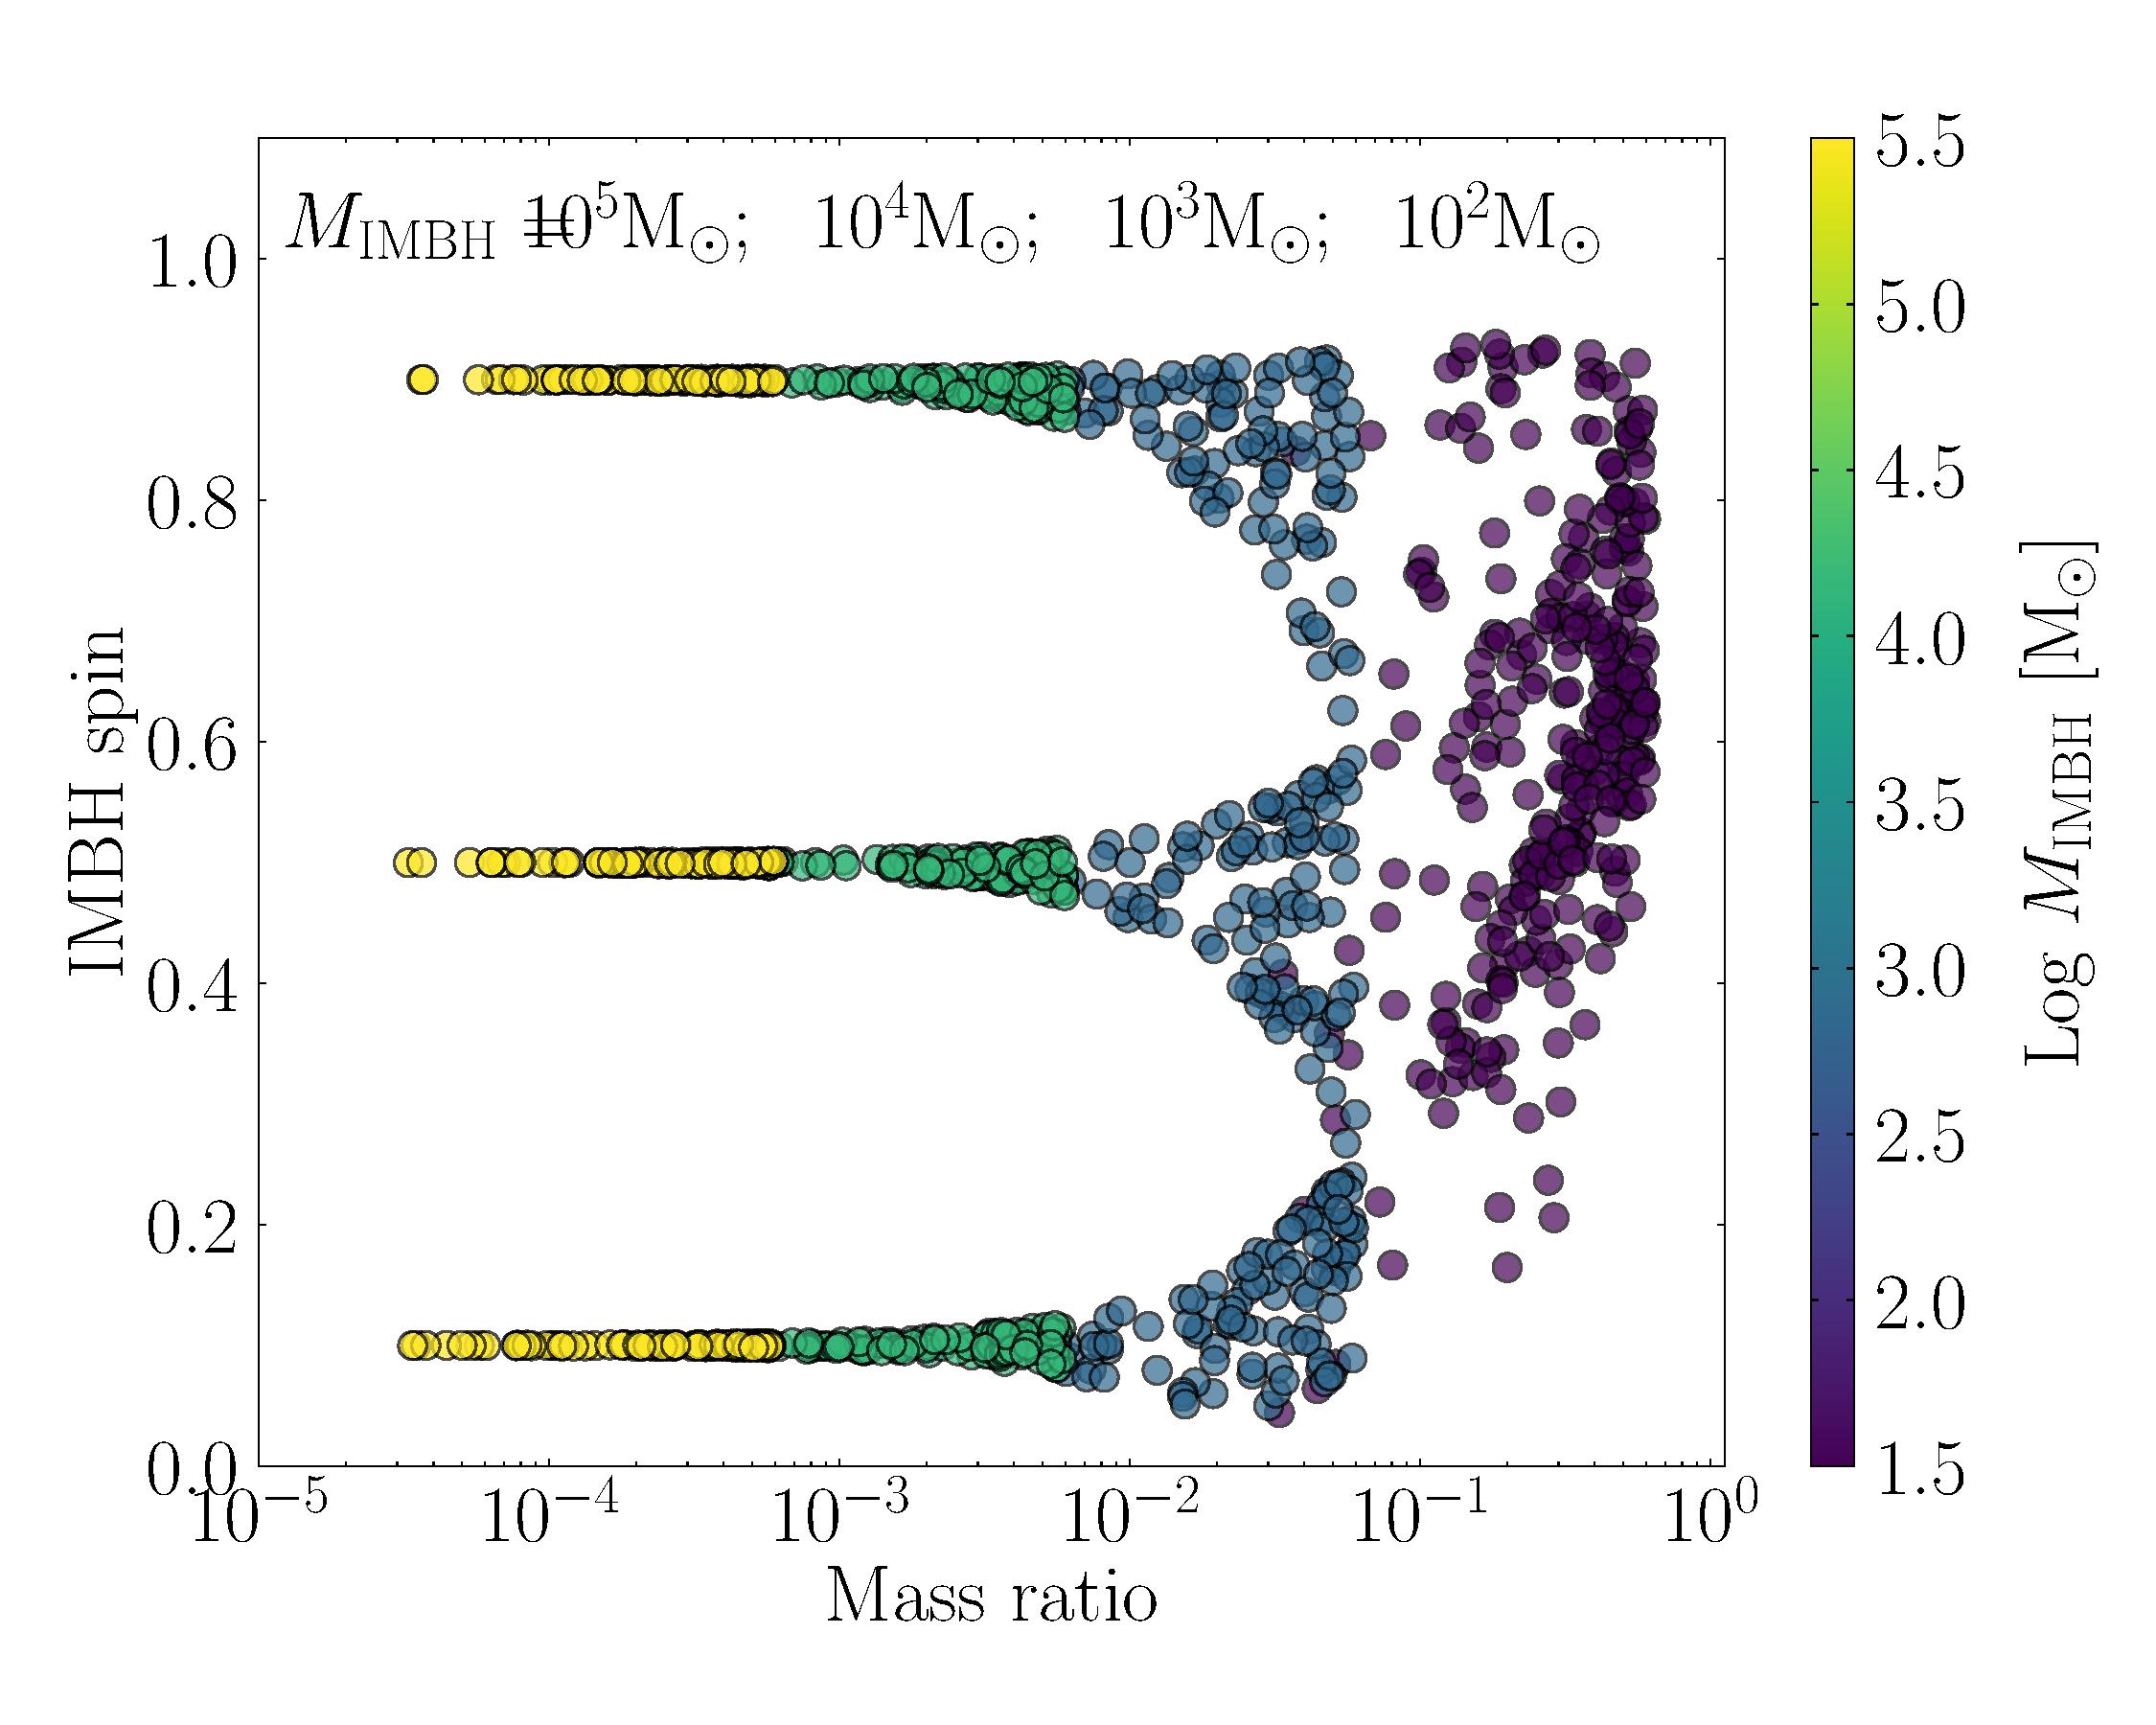
\includegraphics[width=\columnwidth]{track}
\caption{Spin of the IMBH after one merger with a stellar BH as a function of the mass ratio. Different colors identify different values of the IMBH.}
\label{fig:f11a}
\end{figure}

\begin{figure}
\centering
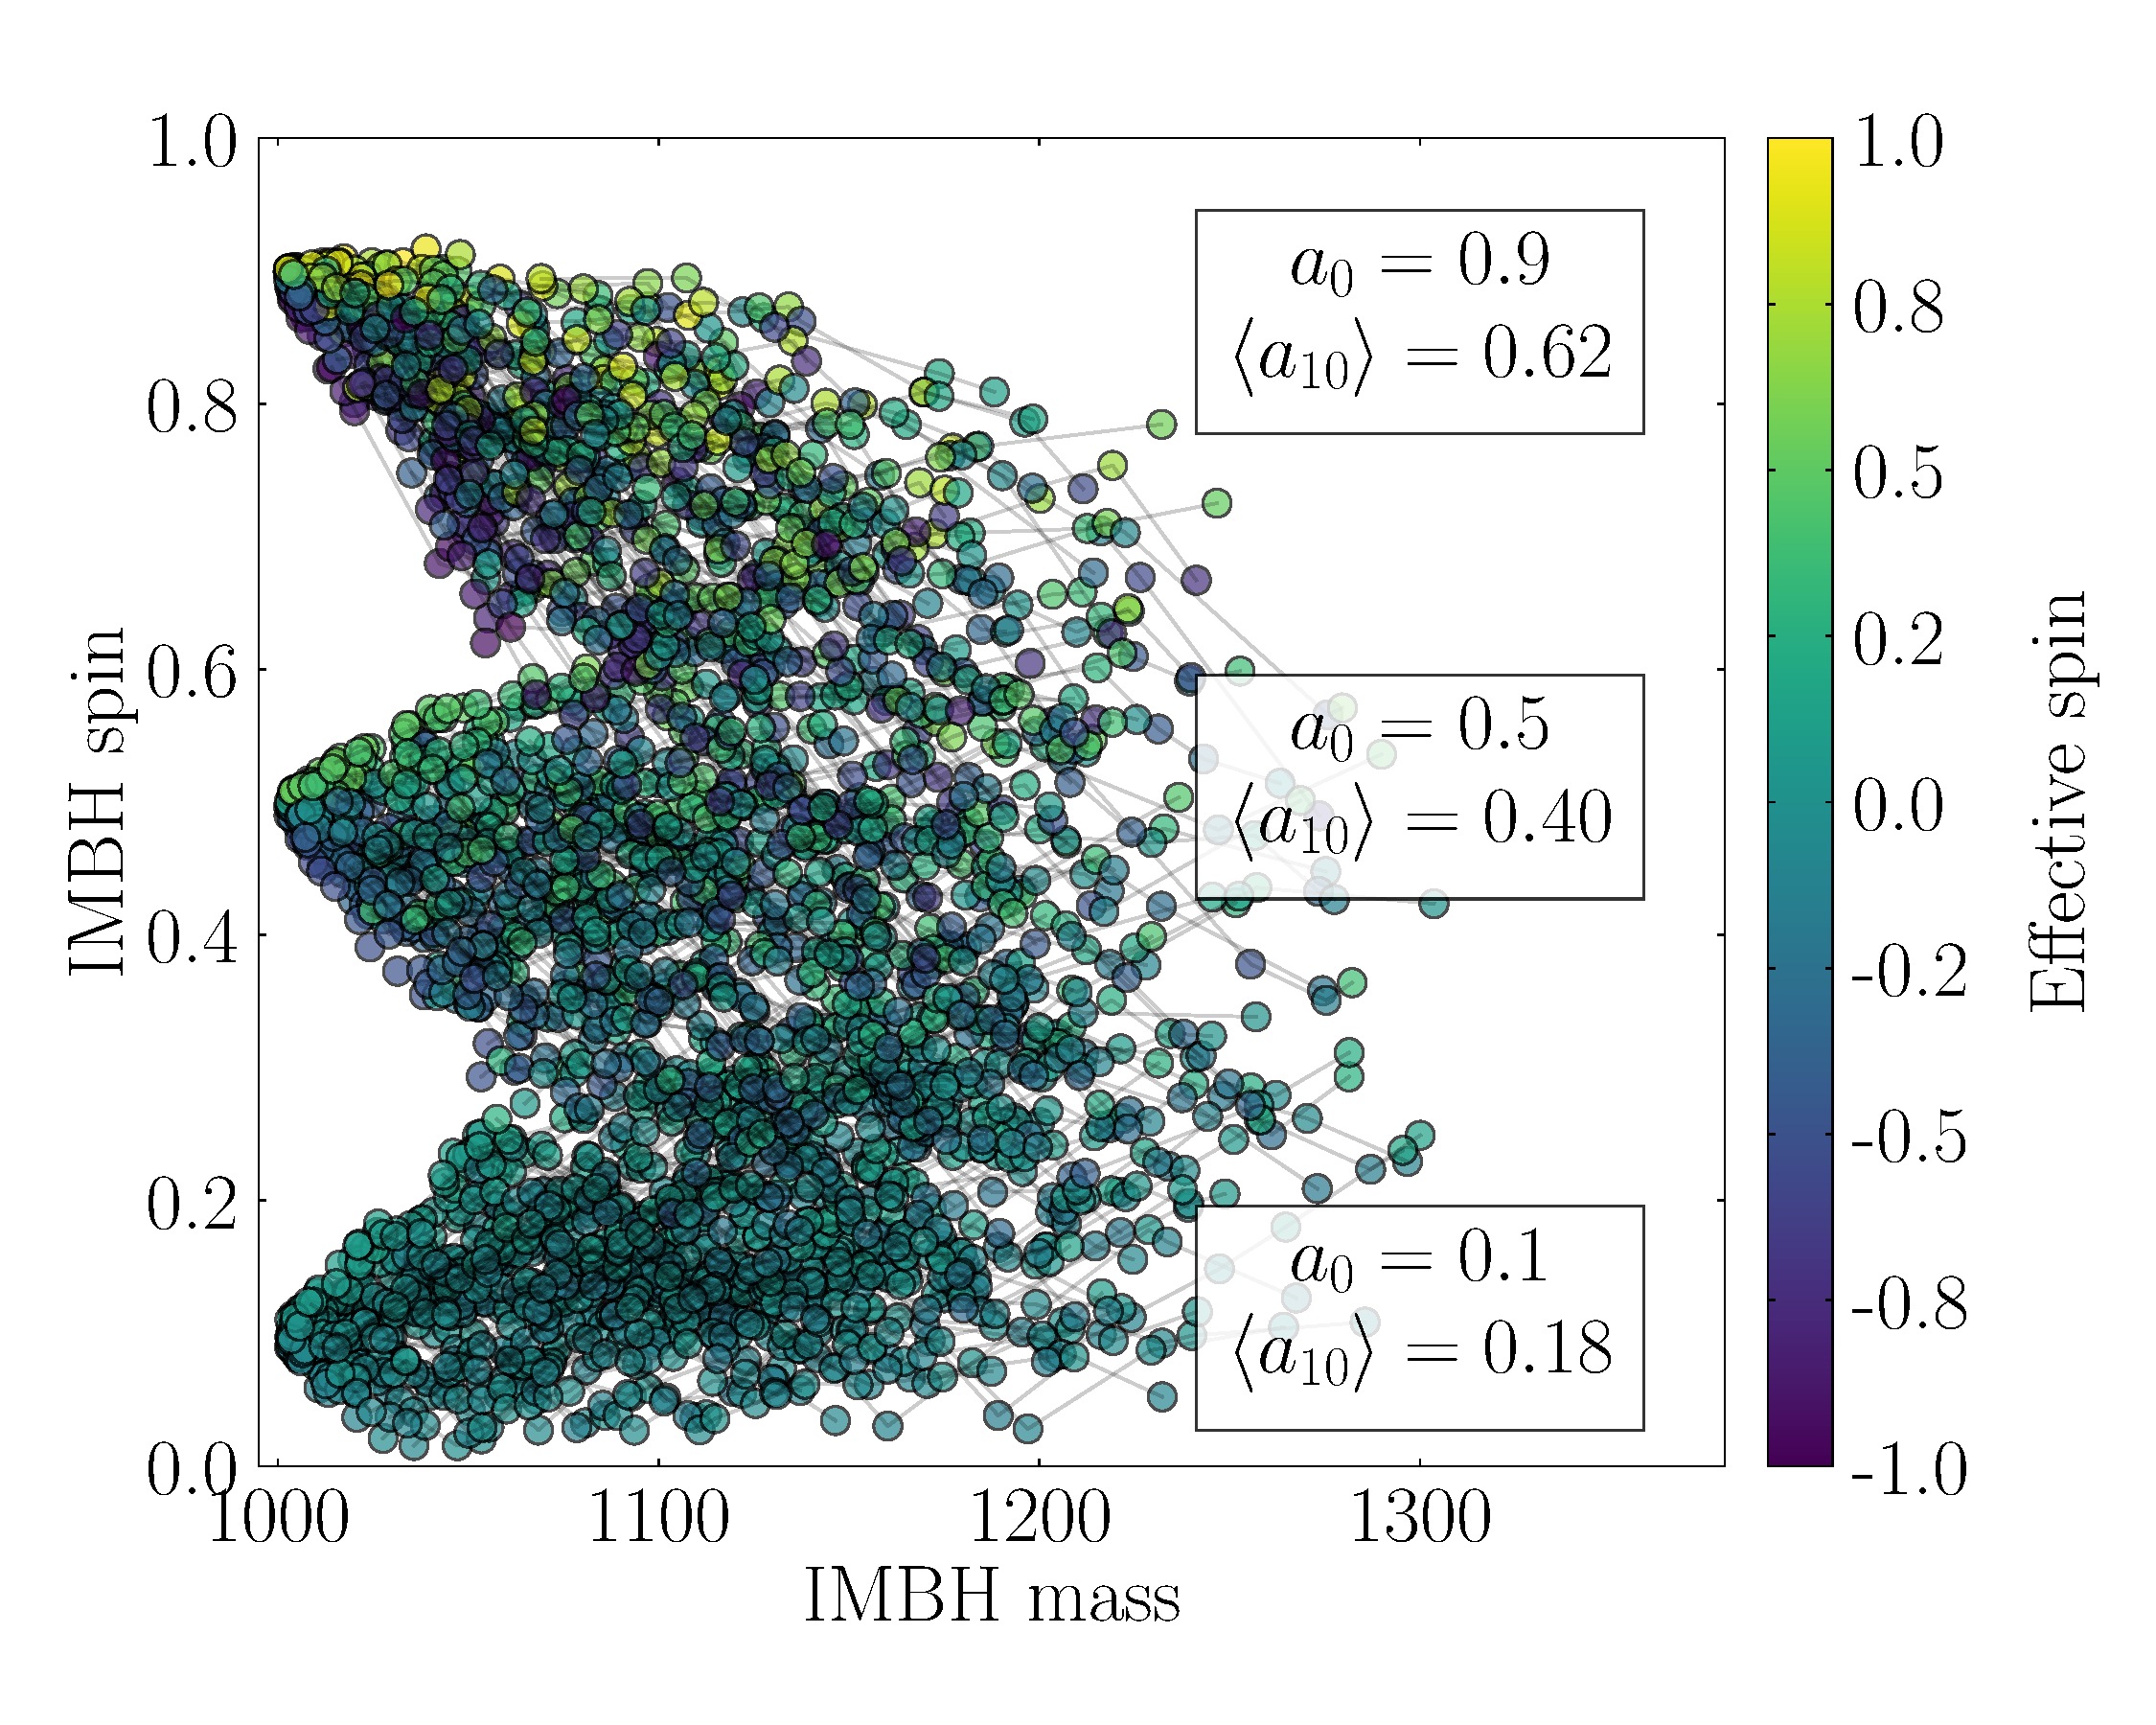
\includegraphics[width=\columnwidth]{track1000}
\caption{Spin evolution for an IMBH with initial mass $M_\ibh = 10^3\Ms$ and initial spin either $a_0 = 0.1$, $0.5$, or $0.9$ that undergoes 10 consecutive mergers with stellar mass BHs. For each value of $a_0$ we run 100 different merger trees, each shown in the plot
as connected by a thin black line. The colour-coding marks the effective spin parameter calculated at each IMBH-BH merger. The labels  show the initial value of the IMBH spin adopted, and the average value of the spin after the 10th merger. }
\label{fig:f11b}
\end{figure}


\section{Gravitational waves}
\label{gra}

\subsection{Gravitational wave signal}
{\bf
Our simulations encompass a wide range of IMRI models, in fact touching the layer of ``ordinary'' BH binaries (mass ratio $q>0.1$) and 
scratching the limit of extreme-mass ratio inspirals ($q < 3 \times10^{-5}$). This setup implies that the GW emission connected with our modelled mergers can populate a wide range of frequencies, from milli- to deca-Hz. Figure \ref{fig:f13} show the characteristic amplitude as a function of the frequency for a sample of IMRI mergers with different IMBH mass, assuming they are located at redshift $z=0.1$ ($\sim 460$ Mpc) and an observation time of 4 yr. We compare the modelled signal with the sensitivity curve of several detectors, namely LISA, ALIA, DO, DECIGO, LIGO, and the Einstein Telescope (ET). We see that mergers involving IMBHs with masses $< 10^5\Ms$ are promising multiband sources that can be seen in one detector during the inspiral phase and in another during the merger. The number of regions in which a detector is sensitive traversed by an IMRI widens at increasing the IMBH mass, in fact in principle an IMBH with mass $<10^3\Ms$ can be seen across the whole milli-decaHz frequency range.  

\begin{figure}
\centering
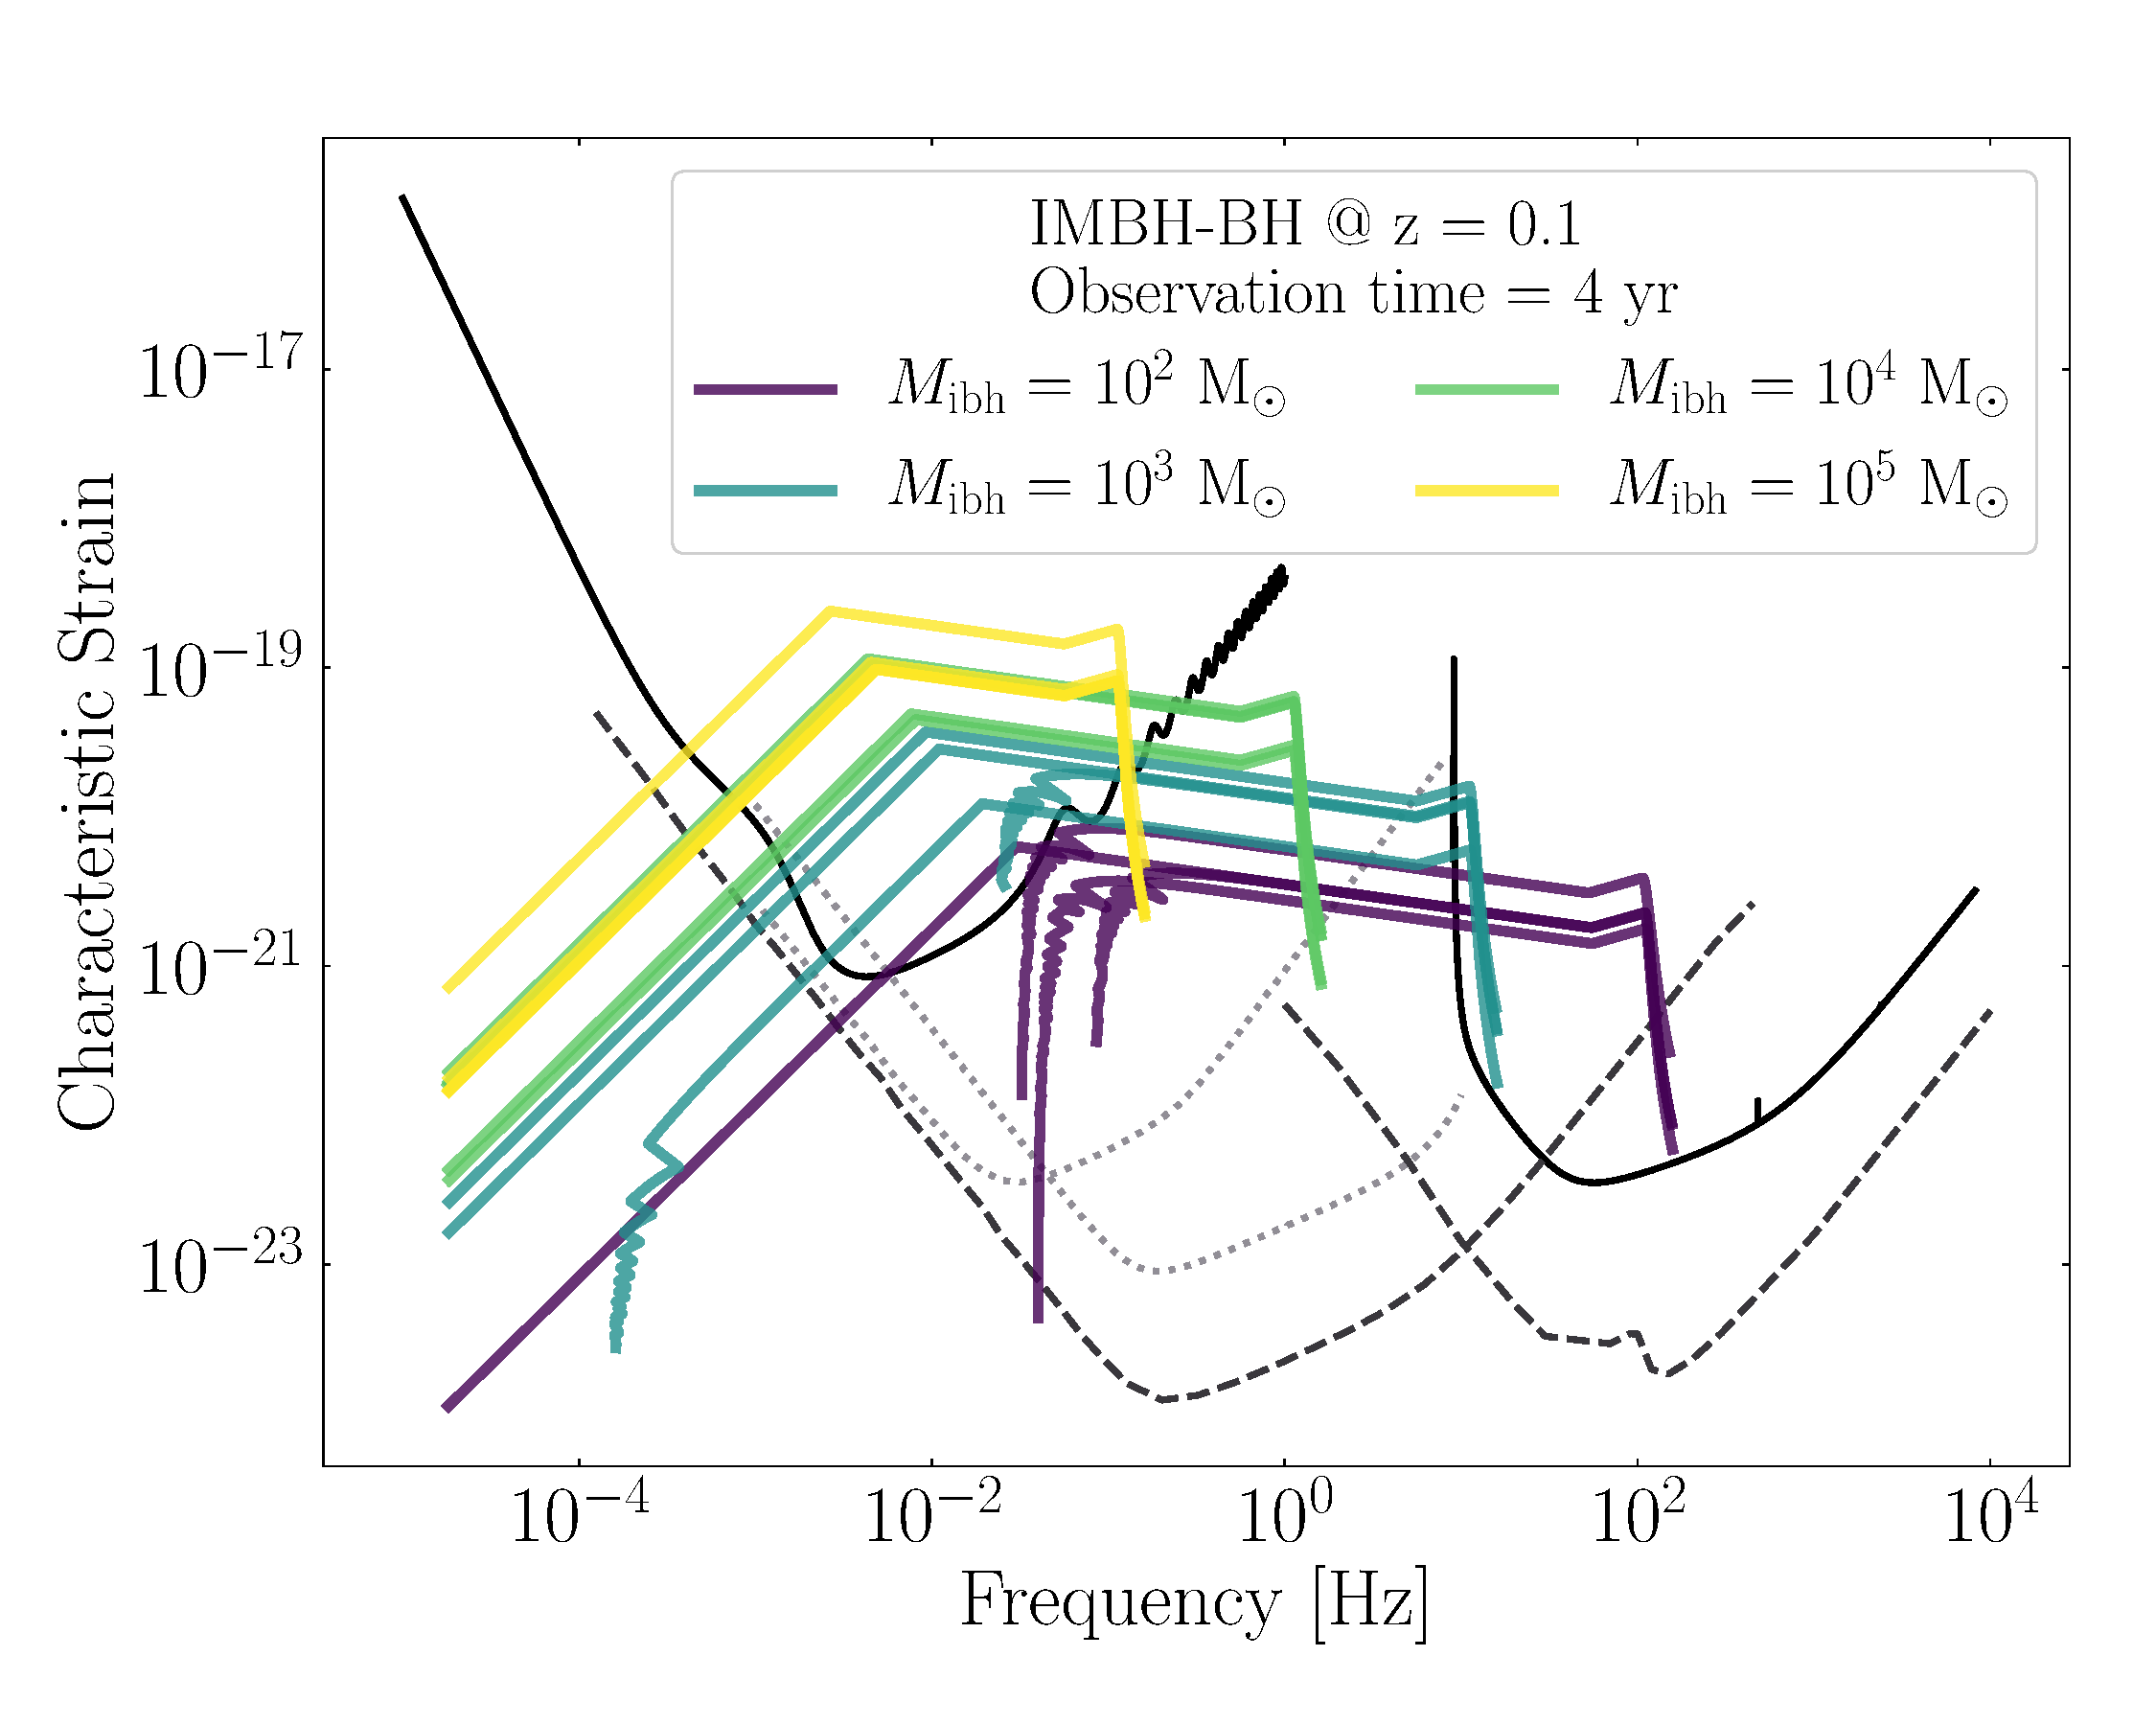
\includegraphics[width=\columnwidth]{test}
\caption{Characteristic strain - frequency evolution for a sample of mergers in SET0. Each point in the plane refers to the signal associated with the IMRI dominant frequency. Different colors identify different IMBH mass ($M_\ibh$). The calculated signal is overlayed to the sensitivity curve of several detectors, from lower to higher frequency: LISA and LIGO (straight black line), DECIGO and Einstein Telescope (dashed black line), ALIA and Decihertz Observatory (dotted black lines).}
\label{fig:f13}
\end{figure}

}

\subsection{Eccentricity of IMRIs}
{\bf
One important parameter that could be inferred from GW observations is the eccentricity of the source. To better understand whether our IMRI models are expected to retain a significant eccentricity while transiting across different observational bands, we show in Figure \ref{fig:f10} the average value of the eccentricity calculated when IMRIs cross the milli-Hz, deci-Hz, and Hz bands for all simulations set. It is apparent that even when emitting low-frequency GWs, IMRIs have already significantly circularized, although apparently lower-mass IMRIs tend to have slightly larger eccentricities. The fact that our IMRIs are substantially circular when becoming observable to GW detectors has implications on their detectability, as we show in the next section.
}

\begin{figure}
\centering
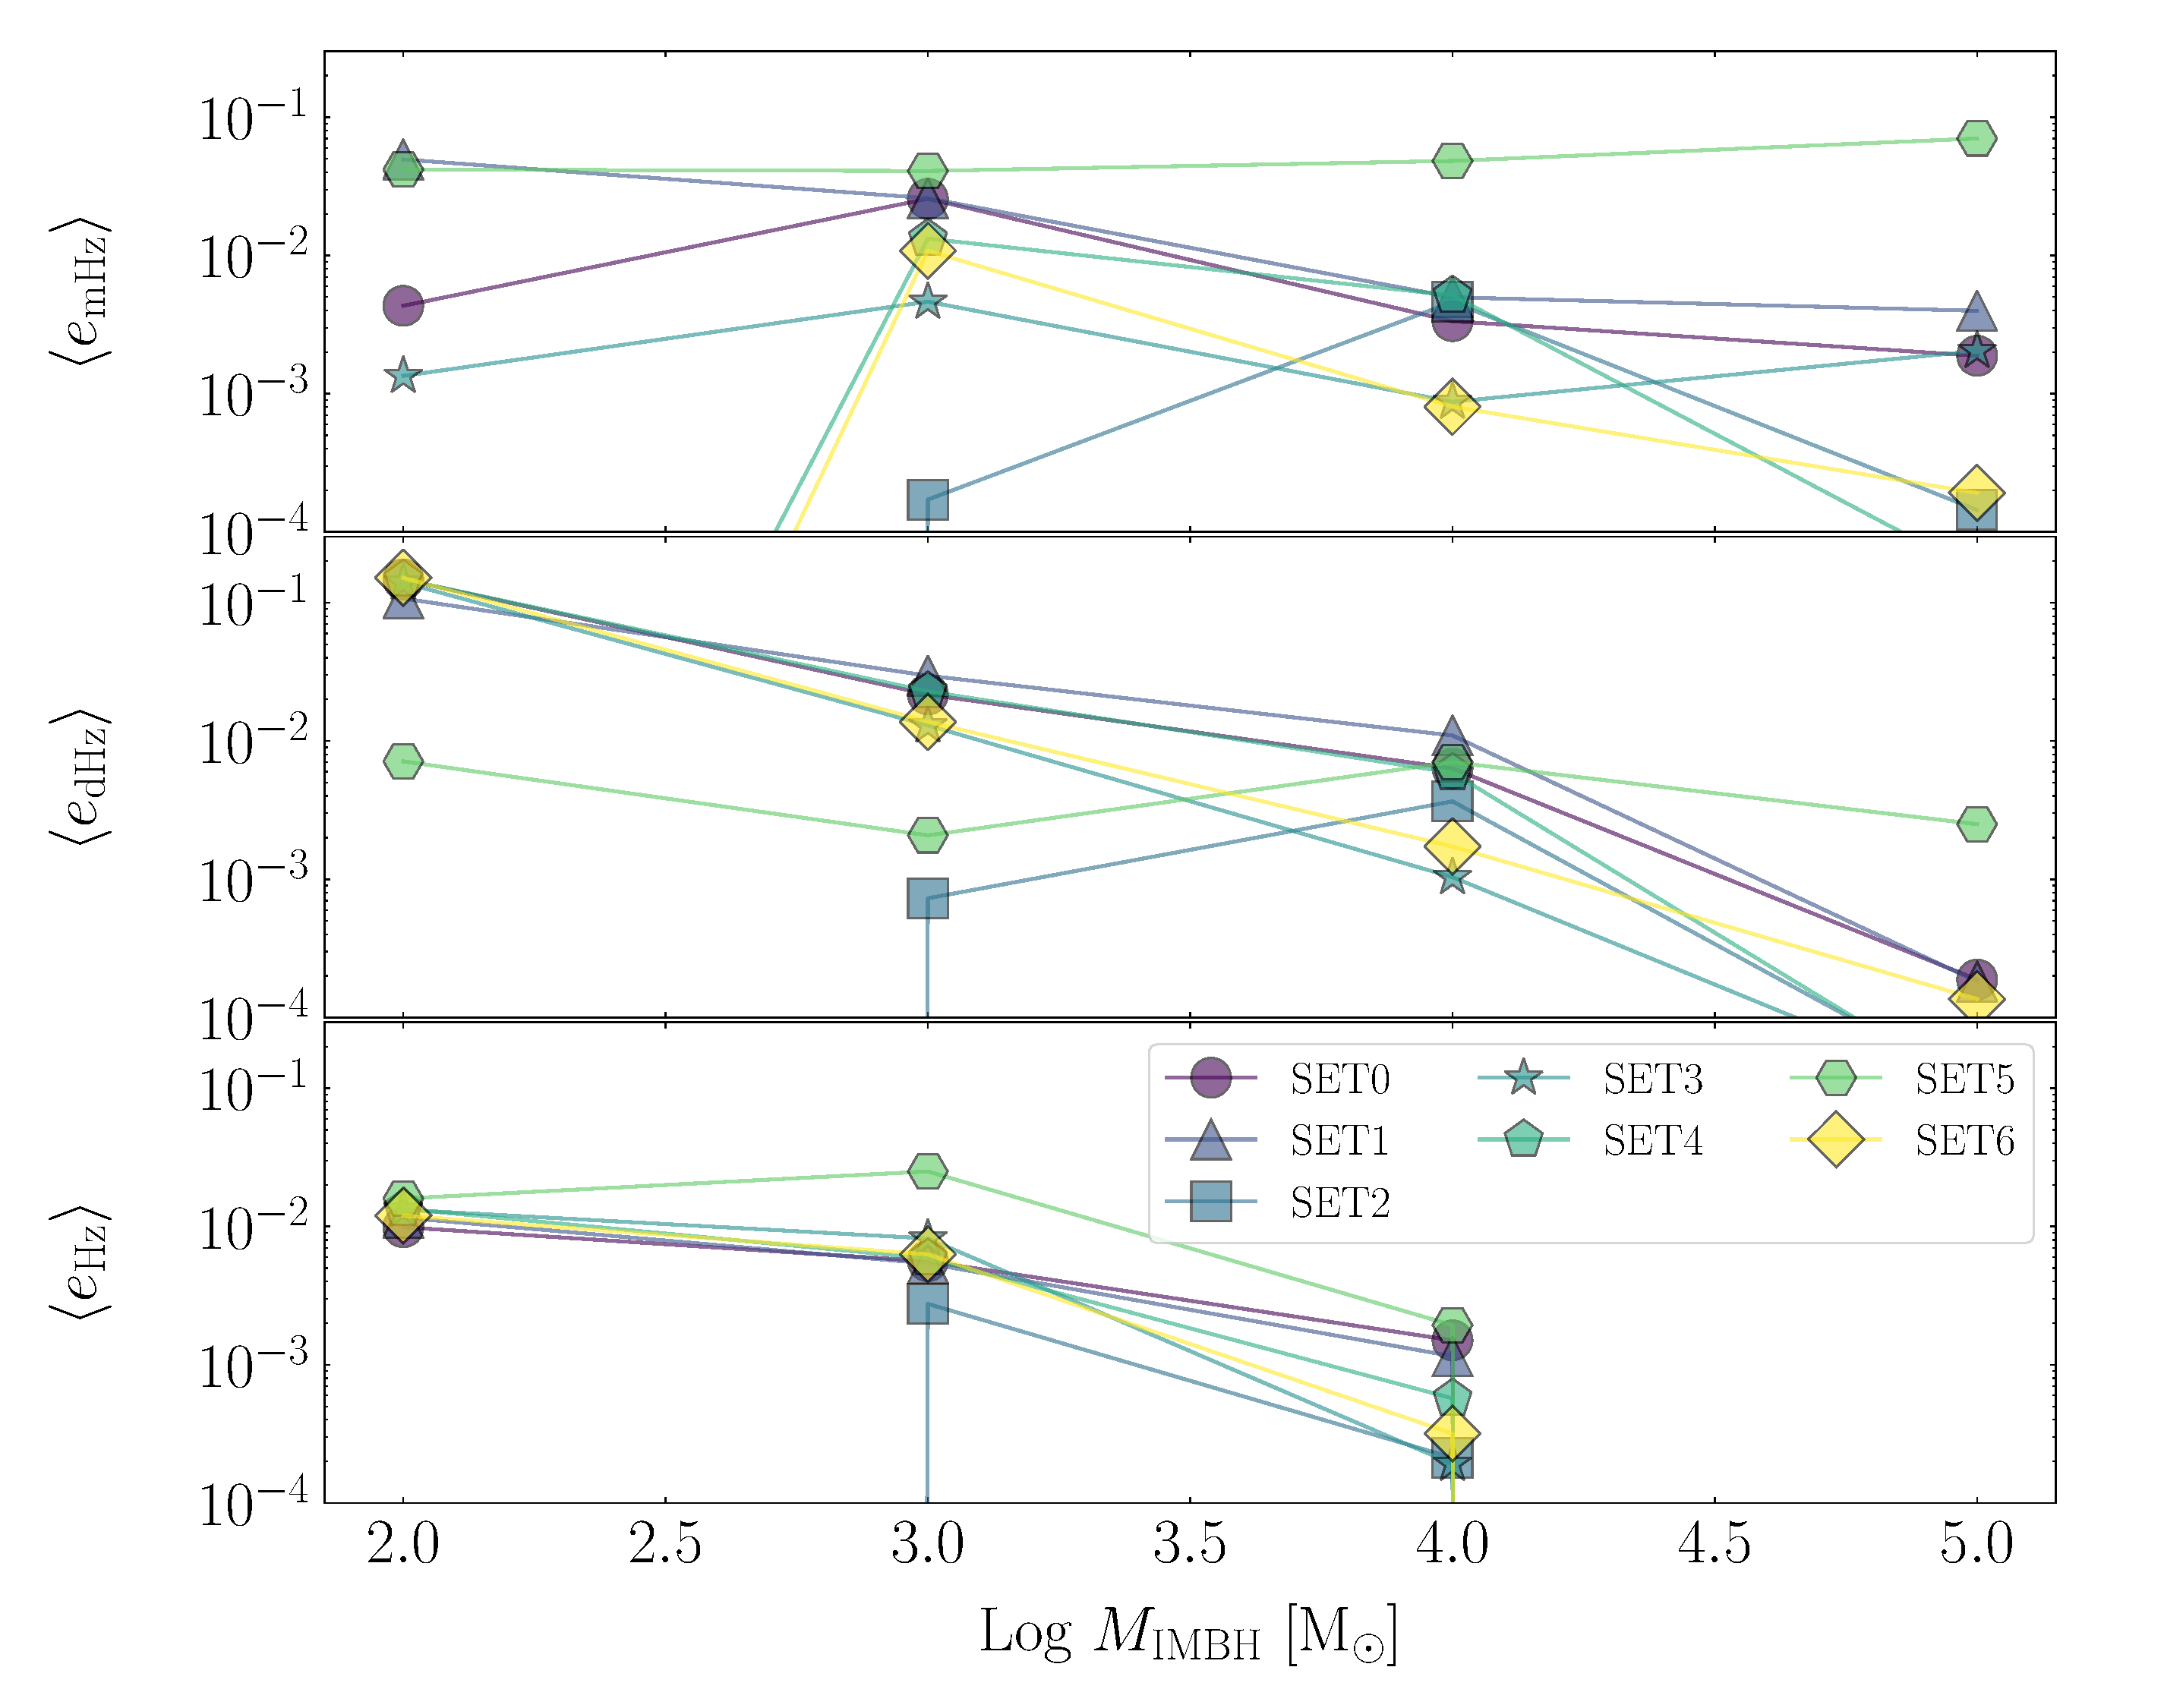
\includegraphics[width=\columnwidth]{averageec}
\caption{Average eccentricity of IMRIs emitting in millihertz (top panel), decihertz (central panel), and Hertz (bottom panel). Different colors and symbols identify different models. }
\label{fig:f10}
\end{figure}



\subsection{Detecting IMBHs in Milky Way globular clusters and in the Large Magellanic Cloud}

In this section, we exploit our results to investigate whether the current design of LISA provide enough sensitivity to unveil the presence of IMBHs in our closest neighbourhood. 
To perform such a study, we assume to have a nearly circular IMRI with an IMBH mass in the range $10^2-10^6\Ms$ and a BH companion weighing either $10$ or $30\Ms$. 
We assume that the IMRI emission frequency is 1 mHz, corresponding to an orbital semimajor axis $10^{-3}-10^{-2}$ AU. 
The merger time for IMRIs in this configuration ranges between $100$ and $10^4$ yr, thus much larger than the observation time. Assuming 4 yr observation time, the IMRI frequency will not vary sensibly, being the frequency variation $\Delta \ln f < 10^{-4}$. As noted by \cite{robson19}, whenever the latter quantity remains below 0.5, a GW source should be treated as nearly stationary. Upon this assumption, the signal-to-noise (SNR) ratio can be written as
\begin{equation}
    {\rm SNR}^2 = h_{\rm GB}^2 f / h_n,
\end{equation}
where $f$ is the source initial frequency, $h_n$ is the adimensional instrument sensitivity, and 
\begin{equation*}
    h_{\rm GB} = \frac{8T_{\rm obs}^{1/2} (G\mathcal{M}/c^3)^{5/3} (\pi f)^{2/3}}{\sqrt{5}D_L/c},
\end{equation*}
with $T_{\rm obs}$ the observation time, $\mathcal{M}$ the IMRI chirp mass, and $D_L$ the luminosity distance. Note that the relation above implies that the SNR scales with $D_L^{-1/2}$.
Figure \ref{SNRMW} shows the SNR calculated for the LISA instrument for IMRIs having an initial frequency $f=1$ mHz and masses in the $10^2-10^6 \Ms$ range, assuming a luminosity distance of $D_L = 8$ kpc. 
We find that an IMRI with mass $M_\imri = (30 + 10^3)\Ms$ has an associated SNR of 20, whereas this quantity rises up to 100 for a $10^4\Ms$ IMBH. 
These estimates suggest that LISA can play a crucial role in probing the existence of IMBHs in the Galactic backyard. 
\begin{figure}
    \centering
    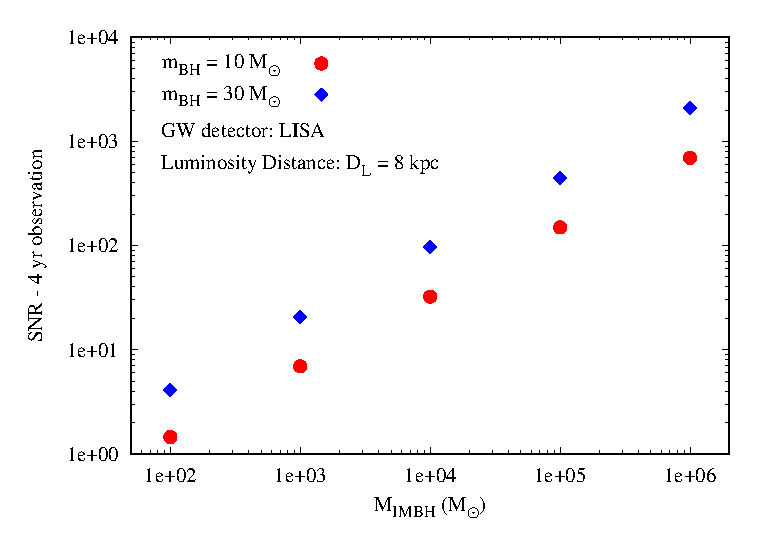
\includegraphics[width=\columnwidth]{snr_MW}
    \caption{SNR for several IMRIs assuming an initial frequency of $1$ mHz, 4 yr of observation time, and a luminosity distance of $D_L = 8$ kpc.}
    \label{SNRMW}
\end{figure}

{\bf In fact, in the last decade a number of works pointed out the potential presence of IMBHs in Galactic globular clusters, although in most cases the results were inconclusive. Concerning clusters orbiting closer than 8 kpc to us candidates include: 47Tuc \citep{kiziltan17}, NGC6266 \citep{abbate19}, NGC6128 and NGC288 \citep{sollima16}, NGC6388 and NGC2808 \citep{miocchi07,lanzoni07}.
For instance, the inferred value for the 47Tuc IMBH mass goes from $M_\ibh > 2,000\Ms$ \citep{kiziltan17} to substantially lower values $\ll 1,000\Ms$ \citep{abbate19b}, depending on the observational technique adopted. A similar discussion involves other clusters, like NGC6388 \citep{lanzoni13,lutzgendorf13}. Therefore, LISA might play a crucial role in unravelling the presence (or not) of IMBHs in the Galaxy, at least the closest one.

Not only, in fact LISA can also be used to provide clues about the presence of IMBHs in nearby galaxies. For instance, it has been recently suggested that the Large Magellanic Cloud might be harbouring an IMBH with a mass in the range $4\times 10^3-10^4\Ms$ \citep{erkal19} and up to $10^7\Ms$ \citep{boyce17}, and that some of the clusters residing in the cloud can host IMBHs as well with masses in the range $10^3-10^4\Ms$ \citep{gualandris07}. Assuming a distance to the LMC $D_L = 49.97 \pm 1.13$ kpc \citep{pietrzy13}, we find that LISA might deliver observations of {\it Magellanic} IMRIs with an $SNR = 8-40$, with the lower(upper) value corresponding to an IMBH with mass $10^3\Ms$($10^4\Ms$) and a BH companion of $30\Ms$. 
}




\subsection{IMRIs merger rate}
%{\color{red} TO BE REVISED EVERYTHING BELOW!\\
%In particular, the discussion about the MW needs to be completely reshaped because the power-law approximation is no longer valid. We could use 
%an approximate stuff like 35./180. GCs might have an IMBH with mass 1,000 thus probability for IMRI is X, thus the probability for the MW is tot, thus
%the probability for MW analogs is tot, something like this could be ok-ish.
%}
%
%Previous studies based on full consistent N-body simulations of star clusters containing IMBHs with various masses and general properties  \citep{konstantinidis13,haster16,leigh14, macleod16} have shown that binary formation involving an IMBH takes place at a rate of $R_{\rm bin} \sim 10^{-7}$ yr. Assuming typical ages for globular-like star clusters of $t_{\rm age}\sim 10^{10}$ yr and assuming that IMBH buildup occurs in the clusters early lifetime ($\lesssim 1$ Gyr), we can use the merger probability fitting function depicted in Equation \ref{fmerg} to infer the total number of IMRIs formed for a given IMBH mass and over a cluster lifetime $t_{\rm age}$
%\begin{equation}
%    N_\gc(M_\ibh) = R_{\rm bin}t_{\rm age}f_{\rm mer} \sim 15\left(\frac{M_{\ibh}}{10^2\Ms}\right)^{0.38},
%\end{equation}
%ranging from $\Gamma_{\imri} = 15-90$ yr$^{-1}$ for $M_\ibh = 10^2-10^4\Ms$, respectively.
%To put such a quantity in the context of MW-like galaxies, we need to make assumptions on the IMBH putative mass function. Assuming that the initial mass function of GCs follows a power-law and exploiting Equation \ref{mcmibh}, we can write the IMBH mass function as $f(M_\ibh) = k (M_\ibh/10^\alpha)^{1/\beta}$. The normalization constant $k$ can be calculated by assuming that the mass in clusters constitute a fraction of the total galaxy mass:
%\begin{equation}
%k = \frac{\delta M_g (2-s)}{(M_{\gc 2}^{2-s} - M_{\gc 1}^{2-s})},
%\label{normal}
%\end{equation}
%with $\delta = 5\times 10^{-4}$ \citep{webb15,belczinski17}, $M_g = 6\times 10^{10}\Ms$ the Milky Way stellar mass, and $M_{\gc 1,2} = (5\times 10^3 - 8\times 10^6)\Ms$ the range of GC initial mass. 
%Combining equations above, we can infer the total number of IMRIs  MW-like galaxies as
%\begin{align}
%    N_{\rm MW} =& f_\ibh N_\gc \int_{M_{\ibh ,1}}^{M_{\ibh ,2}} \Gamma(M_\ibh) \times \nonumber \\
%    & \times f(M_\ibh) \frac{\derd M_\gc}{\derd M_\ibh} {\rm d}M_\ibh,
%\end{align}
%where $f_\ibh N_\gc$ is the number of GCs containing an IMBH, and the term $\derd M_\gc / \derd M_\ibh$ is used to perform a change of variable from the GC to the IMBH mass. The integral has analytical solution in the form
%\begin{equation}
%N_{\rm MW} = K \frac{M_{\ibh ,2}^{\beta + b(1-s)} - M_{\ibh ,1}^{\beta + b(1-s)}}{\beta + b(1-s)},
%\end{equation}
%with the parameter $K$ containing all the constant factors.
%Assuming $t_{\rm age} = 10$ Gyr and in the IMBH mass range of $10^2 - 10^4\Ms$, we derive an IMRI merger rates for MW-like galaxies of
%\begin{equation}
%\Gamma_{\rm MW} = 2.26\times 10^{-5} {\rm ~yr} \left(\frac{10{\rm ~Gyr}}{t_{\rm age}}\right)\left(\frac{f_\ibh}{0.2}\right)\left(\frac{N_\gc}{180}\right).
%\label{eqMW}
%\end{equation}
%The number of MW-analogs in the local Universe (redshift $z<0.1$) is roughly proportional to the luminosity distance $D_L$, namely $P_{\rm MW} = 4\pi/3 \times 0.0116(2.26)^{-3}D_L^3$ with $D_L$ expressed in Mpc \citep{abadie10}. Thus a rough estimate of potential IMRIs developing in MW-like galaxies in the local Universe is given by $\Gamma_{\rm MW} \times P_{\rm MW} = 10.5$ yr$^{-1}$.
%This is a simple estimate, though, which not account for the distribution of galaxies across different redshift or the actual volume within which a detector is sensitive.

The launch of the LISA detector and the start of operations of the next generation of GW observatories like the Einstein Telescope (ET) will enable us to observe this kind of objects at cosmological distances. Therefore, to infer the IMRI merger rates, we need to take into account in our calculation how the number density of galaxies varies across redshift $z$.
The GW source {\it horizon} determines the maximum distance in space, or the redshift $z_{\rm hor}$, at which the source signal is detected with a threshold signal-to-noise ratio (SNR), namely:
\begin{equation}
{\rm SNR^2} = \int_{f_1}^{f_2} \displaystyle{\frac{h_c^2(f,z_{\rm hor})}{S_n^2(f)}} {\rm d}f,
\end{equation}
with $f_{1,2}$ the initial and final frequency of the GW signal, $h_c(f,z)$ its characteristic strain, and $S_n(f)$ its sensitivity. To determine this quantity, we integrate the final stage of the IMRI signal assuming an observation time of 4 yr -- i.e. the nominal duration time of the LISA mission -- and we calculate the value of $z_{\rm hor}$ at which we get an SNR of 15. We assume the set of cosmological parameters measured by the Planck mission, namely $H_0 = 67.74$ km/s/Mpc$^{3}$, $\Omega_m = 0.3089$, $\Omega_\Lambda = 0.6911$ \citep{planck15}. To calculate $z_{\rm hor}$, we vary the IMBH mass in the range $50-10^6\Ms$ assuming that the companion has a mass of either $10$ or $30\Ms$. Figure \ref{fig:fhor} shows how the horizon redshift changes for four different detectors: the Laser Interferometer Space Antenna \citep[LISA\footnote{\url{https://www.elisascience.org/}},][]{amaro12}, the Deciherz Gravitational-Wave Observatory \citep[DECIGO\footnote{\url{http://tamago.mtk.nao.ac.jp/spacetime/decigo_e.html}},][]{seto01}, the Einstein Telescope \citep[ET\footnote{\url{http://www.et-gw.eu/}},][]{punturo10}, and LIGO. 


\begin{figure}
\centering
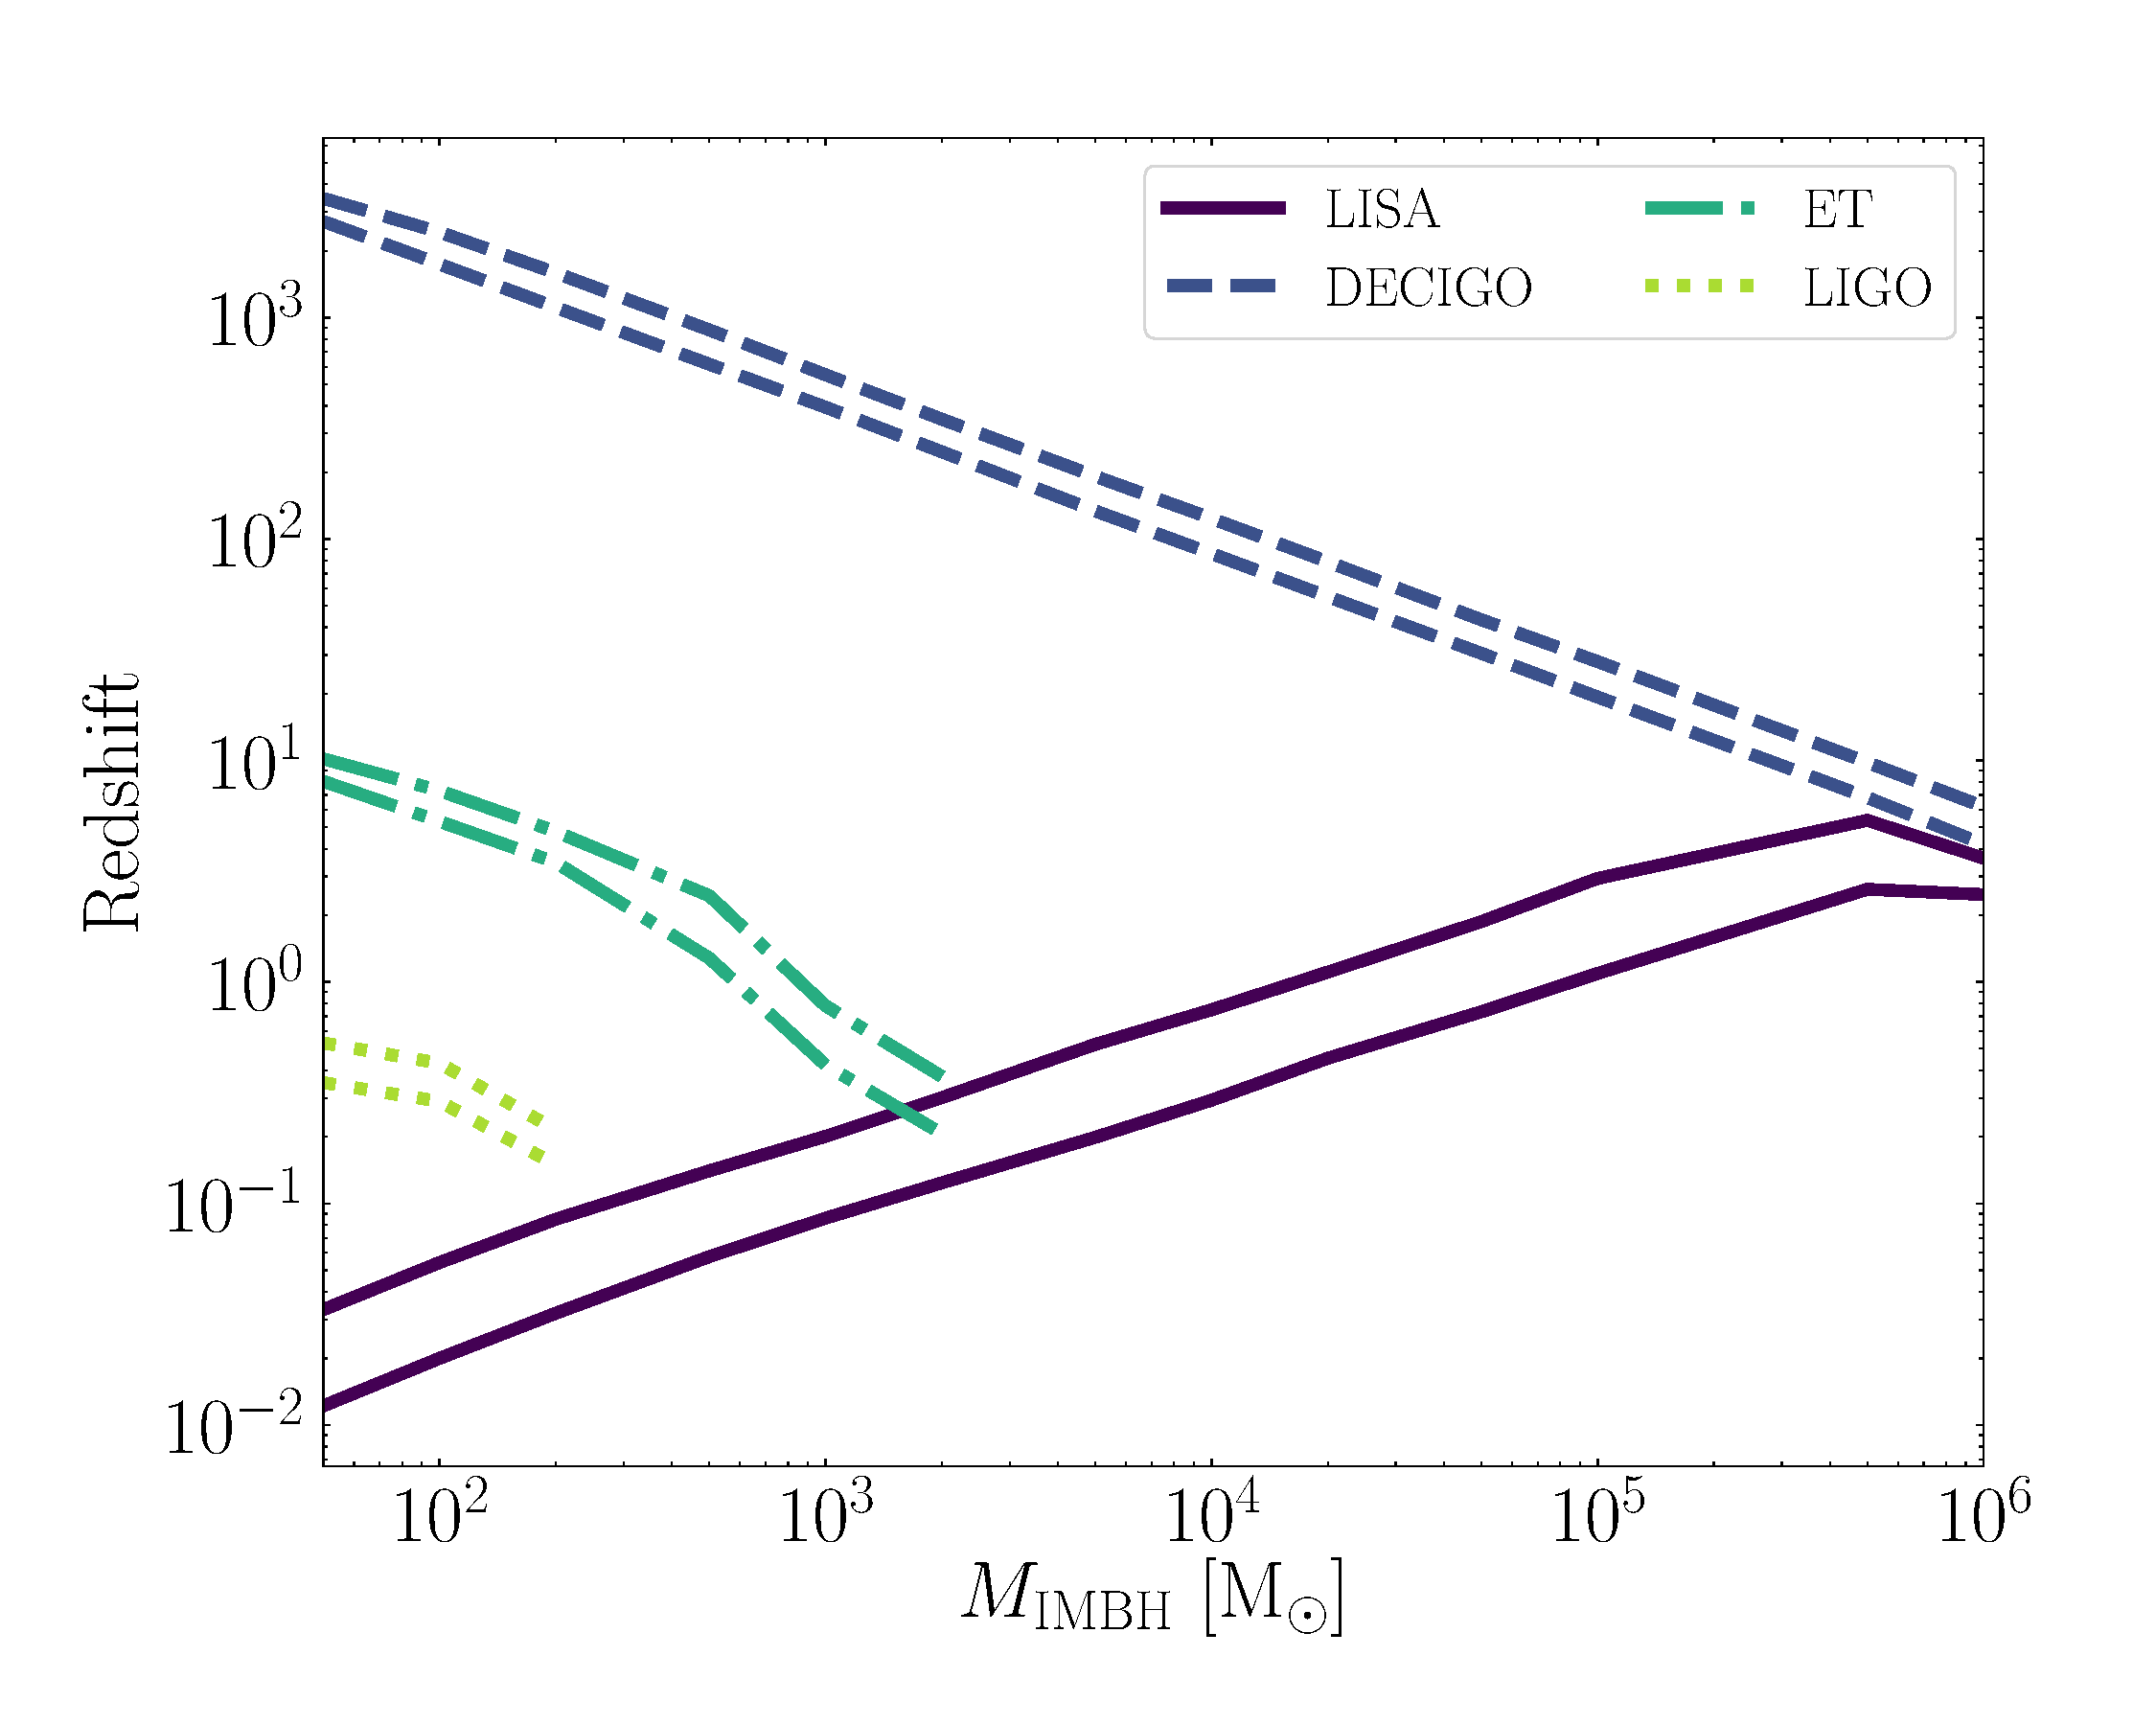
\includegraphics[width=\columnwidth]{horizon}
\caption{Horizon redshift as a function of the IMBH mass assuming a BH companion with mass $10 \Ms$ (lower curves) or $30\Ms$ (upper curves). Different curve collections correspond to different detectors: LISA (straight lines), DECIGO (dashed lines), ET (dotted lines), LIGO (dot-dashed lines). In the next section, we discuss whether some classes of IMRIs can appear as multiband sources}.
\label{fig:fhor}
\end{figure}

From the plot is evident that ground based telescopes provide a relatively limited view on the IMBH realm, although LIGO can provide insights on low-mass IMRIs ($<500\Ms$) up to redshift $z_{\rm hor} \leq 0.2$ and ET will enable the observation of IMRIs with mass $<10^3\Ms$ up to $z_{\rm hor} = 1-10$, the same range of redshift accessible with LISA to listen GWs from heavy IMRIs ($M_{\imri}>10^4\Ms$). Decihertz observatories like DECIGO \citep{Kawamura11} and similarly designed mission \citep{arca19}, instead, will allow the detection of IMRIs in the whole $50-10^6\Ms$ mass range up to the dawn of the Universe, thus constituting ideal detectors to unveil the truly nature of IMBHs. 

Once that the dependence between the horizon redshift and the IMBH mass is determined, we can infer the IMRIs rate by calculating the total number of IMRIs inside the cosmological volume encompassed by $z_{\rm hor}$, a requirement that can be expressed as:
\begin{align}
\Gamma_{\imri} = & \Omega_s \int_{M_{1}}^{M_{2}} \int_{0}^{z_{\rm hor}} \frac{\derd n_{\imri}}{\derd M_\ibh\derd z} \times \nonumber \\
& \times \frac{\derd V_c}{\derd z}  \frac{\derd z}{1+z} \derd M_\ibh,
\end{align}
being $\derd V_c/\derd z$ the comoving cosmological volume element, $(1+z)^{-1}$ the term that account for the dilation time, and $\derd n_{\imri}/\derd M_\ibh$ the number of IMRIs per unit of IMBH mass. We can write the latter quantity as
\begin{align}
\frac{\derd n_{\imri}}{\derd M_\ibh} =& \xi_\bh f_{\gw} p_\ibh n_{\rm rep}\times \nonumber \\
& \times \frac{\derd n}{\derd M_g\derd z}\frac{\derd n_\gc}{\derd M_\gc}\frac{\derd M_\gc}{\derd M_\ibh}.
\end{align}
Here, $\xi_\bh$ represents the probability for the IMBH to form a binary with a stellar BH, $\derd n/(\derd M_g \derd z)$ represents the number of galaxies per unit of redshift and galaxy mass, $\derd n/\derd M_\gc$ is the number of clusters per cluster mass in a given galaxy, $\derd M_\gc/\derd M_\ibh$ connects GCs and IMBHs, $n_{\rm rep}$ is the number of times that the same IMBH can form an IMRI with a stellar companion, $f_{\gw}$ is the fraction of IMRIs that undergo merger within a Hubble time (a quantity that is extracted from our simulations, see Figure \ref{fig:gwprob}), and $p_\ibh$ represents the probability for a cluster to host an IMBH. In the following, we assume $p_\ibh = 0.2$ \citep{giersz15}. 

The term $\derd M_\gc / \derd M_\ibh$ can be calculated by inverting Equation \ref{mcmibh} and performing the derivative. For the number distribution of the GCs mass in a given galaxy, $\derd n/\derd M_\gc$, we assume a power-law
\begin{equation}
\frac{\derd n}{\derd M_\gc} = k M_\gc^{-s},
\end{equation}
with the slope $s = 2.2$ and the normalization constant 
\begin{equation*}
k = \frac{\delta M_g (2-s)}{(M_{\gc 2}^{2-s} - M_{\gc 1}^{2-s})}.
\end{equation*}
Assuming Galactic values for the galaxy stellar mass, $M_g = 6\times 10^{10}\Ms$, and star clusters mass range, $M_{\gc 1,2} = (5\times 10^3 - 8\times 10^6) \Ms$, we calculate the corresponding IMBH mass range $M_\ibh \simeq (30 - 4.6\times 10^4)\Ms$ according to Equation \ref{mcmibh}, which can also be used to write $M_\gc^{-s} = aM_\ibh^{-bs}$\footnote{The parameters $a,b$ are obtained manipulating Equation \ref{mcmibh}.}. The $\derd n/(\derd M_g\derd z)$ is obtained exploiting the results in \cite{conselice16}, who studied the distribution of galaxies with stellar masses up to $10^{12}\Ms$ up to redshift $z=8$. In particular, we exploit the following parametric expression of galaxies number density 
\begin{equation}
\phi(z) = -\frac{\phi_* 10^{(\alpha_* + 1)(M_2-M_*)}}{\alpha_* + 1},
\end{equation}
with $\phi_*,~\alpha_*,~M_*$ depending on the redshift \citep[see Table 1 in][]{conselice16}, and $M_2 = 12$. 

Substituting all the terms and manipulating them conveniently, the total number of IMRI in the portion of Universe accessible to a given detector is thus given by
\begin{align}
N_{\imri,1} = & k a^{1-s} b p_\ibh n_{\rm rep} \xi_\bh \times \nonumber \\
& \times \int_{M_{1}}^{M_{2}} \int_0^{z_{hor}} f_{\gw} M_\ibh^{(1-s)b-1}  \derd M_\ibh \times \nonumber \\
& \times   \frac{\phi(z)}{1+z} \frac{\derd V_c}{\derd z}\derd z .
\label{eq:nimri1}
\end{align}

Observations and models suggest that GCs formation peaks at redshift $z=2$, corresponding to a formation time of $t_{\gc ,f} = 3.285$ Gyr. This would imply that the maximum redshift at which a GC containing an IMBH can be observed is the minimum between the horizon redshift and the GC formation redshift. Even in the case in which we assume that GCs forms continuously, we need to set a maximum redshift above which stars did not form yet. Thus, we capped the horizon redshift with either $z=2$ (peak of GC formation), or $z=6$ (formation of the first stars).

The parameter $\xi_\bh$ represents the probability that the IMBH is in a tight binary with a compact remnant. In a typical ensemble of stars with masses following a \cite{kroupa01} initial mass function, the number of stellar BH progenitors is a fraction $\sim 10^{-3}$ of the whole population. In absence of mass segregation and a mass spectrum, we might expect that the probability for an IMBH to be paired with a BH should simply be $10^{-3}$. However, in real systems mass-segregated stellar BHs tend to prevent other stars to migrate into the innermost cluster regions and thus they inhibit the IMBH to capture other stellar types. The direct implication of the dominant effect of stellar BHs on dynamics of the central cluster regions is a high probability for the IMBH to engage a long-term relationship with a stellar BH rather than with a star, thus suggesting $\xi_\bh \rightarrow 1$.


The time over which these IMRI forms can be estimated as the sum of the cluster formation time, the IMBH formation time, the IMRIs formation time, and the IMRI merger timescale:
\begin{equation}
T = t_{\gc ,f} + t_{\ibh ,f} + t_{\imri, f} + t_{\rm GW}. 
\end{equation}
The physics that regulate IMBH formation is still debated and partly unknown. Depending on the formation scenario, models suggest that the IMBH growth can occur either on short ($\sim 1$ Gyr) or long ($\simeq 5-10$ Gyr) timescales. As discussed recently, {\it fast} IMBHs could outnumber those forming slowly \citep{giersz15,AAG19}, thus in our calculations we assume $t_{\ibh ,f} = 2$ Gyr. 
The formation of an IMRI scales with the mass-segregation timescale in the host cluster, which is expected to be of the order of $\sim 0.1-1$ Gyr, while for $t_\gw$ we calculate, from our models, the value at which the number of mergers is half the total number, i.e. $N_\gw(t_\gw) = 0.5 N_\gw$. This corresponds to $t_\gw = 0.6-1.5$ Gyr. 

An alternative way, yet similar, to calculate the merger rate is by exploiting the cosmological GC star formation rate $\rho_{\rm SFR}(z)$, which can be used to calculate the total number of GCs at a given redshift
\begin{equation}
N(z_{\rm max}) =  \int_0^{z_{\rm max}} \frac{\rho_{\rm SFR}(z)}{<M_\gc>}\frac{\derd V_c}{\derd z}\frac{\derd z}{1+z}.
\end{equation} 
Given the power-law GCs mass function used in the previous method, the normalization factor in this case become
\begin{align}
k  =&\frac{(1-s)}{M_{\gc, 1}^{1-s} - M_{\gc ,2}^{1-s}},
\end{align}
and the total number of IMRI inside a given cosmological volume is thus given by
\begin{align}
N_{\imri, 2} = & k a^{1-s} b p_\ibh n_{\rm rep} \int_{M_{1}}^{M_{2}} \int_0^{z_{hor}} M_\ibh^{(1-s)b-1} \times \nonumber \\
& f_{\gw}  \rho_{\rm SFR}(z)\frac{\derd V_c}{\derd z} \frac{\derd z}{1+z} \derd M_\ibh.
\label{eq:nimri2}
\end{align}

We can convert the number of IMRIs in Eqs. \ref{eq:nimri1} - \ref{eq:nimri2} within a given redshift into a merger rate via $\Gamma_\imri = N_\imri / T$. Table \ref{tab:5} summarizes the prospective merger rate calculated for different instruments in units of event per yr.

Assuming a 4 yr long observation run, our estimates suggest that LIGO might be able to detect up to $1-5$ observations of low-mass IMRIs with an IMBH with mass $M_\ibh \simeq 100\Ms$. So far, the three observation runs accomplished by the LIGO-Virgo-Kagra collaboration (LVK), which covers a $\sim 2$ yr time span, seem not to contain such a massive BH, although the loot of detections cumulated during the last run (O3) -- which led to the discovery of around $\sim 60$ new candidates\footnote{\url{https://gracedb.ligo.org/}} -- has not been fully disclosed yet.

At lower frequencies, LISA might record up to $\sim 6-60$ events per yr, pushing the limit for the IMBH mass to up to $40,000\Ms$ and thus allowing to explore the mass range typical of IMRIs $q \simeq 10^{-4}$. 

While the constraints on "present-day" technologies are already quite encouraging, the next generation of both ground- and spaced-observatories could enable us to deliver a much larger amount of observations up to the maximum redshift allowed ($z=2-6$), thus allowning us to probe IMBHs all the way from formation to full growth.

For instance, ET could detected up to $100-800$ IMRIs per yr with masses $M_\imri < 2,000 \Ms$, while space observatories sensitive at decihertz frequencies like DECIGO might record up to $3800$ events per yr.

\begin{table*}
\caption{IMRI merger rate for different detectors }
\begin{center}
\begin{tabular}{cccccccc}
\hline
Instrument & $M_{\rm SBH}$ & $z_{\rm max}$ & $M_{\ibh ,1}$ & $M_{\ibh ,2}$ & $T$ & $\Gamma_1$ & $\Gamma_2$ \\
   & $\Ms$ & &$\Ms$ & $\Ms$ & Gyr & yr$^{-1}$ & yr$^{-1}$ \\ 
\hline
LIGO & $10$ & $0.38$ & $29$ & $200$ & $8$ & $0.81$ &$0.89$ \\
LIGO & $10$ & $0.38$ & $29$ & $200$ & $8$ & $0.81$ &$0.89$ \\
LIGO & $30$ & $0.57$ & $29$ & $200$ & $8$ & $1.89$ &$2.50$ \\
LIGO & $30$ & $0.57$ & $29$ & $200$ & $8$ & $1.89$ &$2.50$ \\
LISA & $10$ & $0.70$ & $29$ & $46240$ & $8$ & $6.01$ &$7.74$ \\
LISA & $10$ & $0.70$ & $29$ & $46240$ & $8$ & $6.01$ &$7.74$ \\
LISA & $30$ & $1.78$ & $29$ & $46240$ & $8$ & $66.40$ &$59.09$ \\
LISA & $30$ & $1.78$ & $29$ & $46240$ & $8$ & $66.40$ &$59.09$ \\
ET & $10$ & $2.00$ & $29$ & $2000$ & $8$ & $140.66$ &$109.04$ \\
ET & $10$ & $6.00$ & $29$ & $2000$ & $8$ & $564.60$ &$215.66$ \\
ET & $30$ & $2.00$ & $29$ & $2000$ & $8$ & $190.53$ &$144.74$ \\
ET & $30$ & $6.00$ & $29$ & $2000$ & $8$ & $812.52$ &$298.68$ \\
DECIGO & $10$ & $2.00$ & $29$ & $46240$ & $8$ & $635.03$ &$486.93$ \\
DECIGO & $10$ & $6.00$ & $29$ & $46240$ & $8$ & $3828.50$ &$1506.62$ \\
DECIGO & $30$ & $2.00$ & $29$ & $46240$ & $8$ & $635.03$ &$486.93$ \\
DECIGO & $30$ & $6.00$ & $29$ & $46240$ & $8$ & $3828.50$ &$1506.62$ \\
\hline
\label{tab:5}
\end{tabular}
\end{center}
\end{table*}








\section{Conclusions}

In this work we studied the dynamical interaction of an IMBH with two stellar BHs under the assumption
that these three massive object dominate completely the dynamics in the innermost regions of a massive star cluster.
We used $28,000$ direct $N$-body models aimed at exploring the formation and evolution of IMRIs, which in this paper we 
broadly define as tight binaries involving an IMBH with mass $> 100 \Ms$ and a stellar BH with mass $\lesssim 50 \Ms$.
In order to assess the role of environments and dynamics on IMRIs formation, we vary the density and metallicity of the 
host cluster, the IMBH mass, the mass spectrum of stellar BHs, and the orbital properties of the three objects. 

Our main results can be summarized as follows:
\begin{itemize}
\item we find that the chaotic interaction between the two BHs and the IMBH favours the formation and merger of IMRIs in a non-negligible fraction of cases. In general, one BH tends to form a more bound binary with the IMBH while the other BH perturbs such a binary. These perturbations are chaotic but can drive the IMBH-BH eccentricity to rise sufficiently for GW emission to kick in, leading to the swift formation
of a merging IMRI [Figure \ref{fig:example}];
\item the merger probability $f_\gw$ increases with the IMBH mass ($M_\ibh$), although in a non trivial way. ``Small'' IMBHs, with mass $M_\ibh \sim 100 \Ms$, have an associated $f_\gw = 5-20\%$ whereas IMRI formation and merger is more frequent for heavier IMBHs, being $f_\gw = 10-60\%$. The large scatter depends mostly on the star cluster density profile and the orbital properties of the IMBH-BH-BH triplet [Figure \ref{fig:gwprob}];
\item our models suggest that the IMRI secondary maps out the overal BH mass distribution. Therefore, the observation of IMRIs would enable us to place constraints on the population of BHs inhabiting the centre of massive star clusters [Figure \ref{fig:mbhdist}];
\item assuming typical values of the cluster velocity dispersion, $\sigma = 5$ km/s for Galactic globular clusters, we show that IMBHs heavier than $M_\ibh \simeq 10^3\Ms$ have $>50\%$ probability to be retained in the cluster after a merger if the companion mass is $<20-30 \Ms$. Lighter IMBHs ($M_\ibh \leq 200\Ms$) are ejected from the cluster whenever the IMRI secondary mass exceeds $10\Ms$. This suggests that an IMBH heavier than $200\Ms$ lurking in the centre of a star cluster has grown more likely via stellar consumption, rather than trhough GW mergers [Figure \ref{fig:survival}];
\item the IMBH spin is another parameter that encodes information about the IMBH evolution. At $M_\ibh>10^4\Ms$, a merger event won't change the IMBH spin, whereas the remnant spin changes significantly if $M_\ibh\simeq10^2-10^3\Ms$. This implies that measuring the IMBH spin prior and after an IMRI can shed a light on the spin distribution of stellar BHs and on the processes that drove the IMBH build-up [Figures \ref{fig:f11a}-\ref{fig:11b}];
\item LISA can help to unravel the presence of IMBHs in our neighbourhood. Assuming a 4 yr long mission, we suggest that LISA can identify IMRIs involving $M_\ibh \sim 10^3-10^4\Ms$ in Galactic GCs, with a signal-to-noise ratio SNR$=10-100$, and in the centre of the Large Magellanic Cloud, where we infer SNR$=8-40$;
\item IMRIs are multiband sources that can be observed with several GW detectors. Assuming 4 yr of observations, we calculate that within the corresponding horizon redshift LIGO can detect up to $0.9-2.5$ events per yr involving an IMBH with mass $M_\ibh \lesssim 200\Ms$. Such a kind of event might have been already recorded during the O3 observation run. LISA has the chance of detecting $6-60$ events yr$^{-1}$ involving $M_\ibh < 46,000\Ms$, whereas the Einstein Telescope ($\sim 10^3$ events yr$^{-1}$ for $M_\ibh < 2000\Ms$) and DECIGO ($\sim 400-3800$ events yr$^{-1}$ for $M_\ibh < 50,000\Ms$) will boost signicantly IMRIs detections, shedding a light on the processes that regulate IMBH seeding and growth at cosmic scales.
\end{itemize}


\clearpage

\section*{Acknowledgements}

MAS acknowledges the Alexander von Humboldt Foundation for the financial
support provided in the framework of the research program "The evolution of
black holes from stellar to galactic scales", and the Sonderforschungsbereich
SFB 881 "The Milky Way System"  -- Project-ID 138713538 -- funded by the German
Research Foundation (DFG).  PAS is indebted with the THAT Group at DESY Zeuthen
for an extended visit, where this work was finished. PAS acknowledges support
from the Ram{\'o}n y Cajal Programme of the Ministry of Economy, Industry and
Competitiveness of Spain.  This work was supported by the National Key R\&D
Program of China (2016YFA0400702) and the National Science Foundation of China
(11873022, 11991053).  The authors acknowledge support from the COST Action
GWverse CA16104. The authors acknowledge the use of the Kepler computer at ARI
Heidelberg, funded by Volkswagen Foundation through the project GRACE 2:
"Scientific simulations using programmable hardware" (VW grants I84678/84680),
and the bwForCluster of the Baden-W\"urttemberg's High Performance Computing
(HPC) facilities, which is supported by the state of Baden-Württemberg through
bwHPC and the German Research Foundation (DFG) through grant INST 35/1134-1
FUGG.

\bibliographystyle{aa}
\newpage
\footnotesize{
\bibliography{ASetal2015}
}


\end{document}
